% !TeX root = ../main.tex
\chapter{Algoritmos del receptor digital}
\label{cap:dsp}
\section{Introducci\'on}
\label{sec:dsp-intro}

En el \cref{cap:transceptor} se obtuvieron las expresiones de las se\~nales
correspondientes a cada uno de los cuatro conversores que componen el
receptor, los cuales digitalizan las componentes en fase y en cuadratura de
las dos polarizaciones ortogonales. En este cap\'itulo se describen los
algoritmos de procesamiento digital implementados en el receptor, encargados
de compensar las degradaciones que introduce el sistema y de realizar la
decisi\'on de s\'imbolo.

En el marco de este proyecto integrador se hace especial \'enfasis en el
algoritmo de recuperaci\'on de frecuencia, ya que es el que fija el l\'imite
de captura del receptor y, por lo tanto, el que determina si el enlace
LEO--GEO resulta viable con el Doppler del \cref{cap:canal}.

\section{Arquitectura de los bloques}
\label{sec:dsp-arquitectura}

La \cref{fig:dsp-cadena} muestra la cadena de algoritmos implementados, desde
la adquisici\'on de las se\~nales hasta la decisi\'on de s\'imbolo final.

\begin{figure}[H]
  \centering
  \resizebox{\linewidth}{!}{%
  \begin{tikzpicture}[
      font=\footnotesize,
      blk/.style={draw, rounded corners=2pt, minimum height=2.6em,
                  text width=6.8em, align=center, inner sep=2pt},
      rx/.style={blk, fill=blue!8},
      bm/.style={blk, fill=orange!12, dashed},
      >={Latex[length=2mm]}]

    \node[rx] (adc)  {ADC\\\scriptsize 2 muestras/s\'imbolo};
    \node[rx, right=0.9em of adc]  (gsop) {Ortogonalizaci\'on\\\scriptsize GSOP};
    \node[rx, right=0.9em of gsop] (foc)  {Recuperaci\'on de frecuencia\\\scriptsize $(\cdot)^4$};
    \node[rx, right=0.9em of foc]  (mf)   {Filtro adaptado\\\scriptsize RRC};
    \node[rx, right=0.9em of mf]   (clk)  {Recuperaci\'on de reloj};

    \node[bm, below=2.6em of clk]  (sync) {Sincronismo con la PRBS};
    \node[rx, left=0.9em of sync]  (eq)   {Ecualizador MIMO\\\scriptsize DD-LMS};
    \node[rx, left=0.9em of eq]    (pll)  {Recuperaci\'on de fase\\\scriptsize PLL};
    \node[rx, left=0.9em of pll]   (dec)  {Decisi\'on};
    \node[bm, left=0.9em of dec]   (met)  {$\BER$ y $\EVM$};

    \draw[->] (adc) -- (gsop);
    \draw[->] (gsop) -- (foc);
    \draw[->] (foc) -- (mf);
    \draw[->] (mf) -- (clk);
    \draw[->] (clk) -- (sync);
    \draw[->] (sync) -- (eq);
    \draw[->] (eq) -- (pll);
    \draw[->] (pll) -- (dec);
    \draw[->] (dec) -- (met);

    \begin{scope}[on background layer]
      \node[draw=blue!45, rounded corners=3pt, inner sep=5pt,
            fit=(eq) (pll)] (lazo) {};
    \end{scope}
    \node[below=0.2em of lazo, font=\scriptsize, blue!45!black]
      {integrados en un solo bloque};

  \end{tikzpicture}}
  \caption[Cadena de procesamiento digital]{%
    Cadena de DSP en el orden en que se ejecuta. En azul, los bloques que
    formar\'ian parte de un receptor de vuelo. En naranja punteado, los dos bloques que utilizan
    la secuencia transmitida: la sincronizaci\'on
    contra la PRBS conocida y el c\'alculo de m\'etricas. El ecualizador y el
    lazo de fase son un solo bloque de c\'odigo, con dos lazos independientes
    adentro.}
  \label{fig:dsp-cadena}
\end{figure}

La cadena consta de seis bloques, cada uno encargado de una degradaci\'on
distinta. El ortogonalizador corrige el desbalance de cuadratura del front end
del receptor. El estimador de cuarta potencia compensa el corrimiento Doppler
de la portadora. El filtro adaptado rechaza el ruido fuera de banda y limita
la interferencia entre s\'imbolos. La recuperaci\'on de reloj corrige el error
de fase de muestreo. El ecualizador MIMO adaptativo compensa la mezcla de
polarizaciones y la interferencia entre s\'imbolos residual. Por \'ultimo, el
lazo de recuperaci\'on de portadora, alojado dentro del mismo ecualizador,
sigue el ruido de fase de los l\'aseres.

Las secciones siguientes describen cada bloque en ese orden. La
justificaci\'on de por qu\'e se eligi\'o ese orden y no otro se desarrolla en
la \cref{sec:dsp-orden}, una vez descriptos todos los algoritmos.

\section{Ortogonalizaci\'on}
\label{sec:dsp-gsop}

\paragraph{Prop\'osito}
Compensa el desbalance de cuadratura del front end del receptor, que hace que
las componentes en fase y en cuadratura de cada polarizaci\'on no sean
ortogonales entre s\'i. El origen de estas imperfecciones est\'a en el
h\'ibrido \'optico de \ang{90} y en la diferencia de ganancia entre los pares
de fotodetectores balanceados.

\paragraph{Principio de operaci\'on}
Se aplica el procedimiento de Gram--Schmidt sobre el par $(r_I, r_Q)$ de cada
polarizaci\'on, donde $r_I$ y $r_Q$ son las se\~nales digitales asociadas a
las componentes en fase y en cuadratura a la salida del
conversor~\cite[ec.~(4.22)--(4.24)]{mello2021}. Se toma $r_I$ como
referencia, se le resta a $r_Q$ su proyecci\'on sobre $r_I$ y se renormaliza,
\begin{equation}
  r_I^{\mathrm{ort}} = \frac{r_I}{\sqrt{\E{r_I^2}}},
  \qquad
  r_Q^{\mathrm{int}} = r_Q - \frac{\E{r_I r_Q}}{\E{r_I^2}}\, r_I,
  \qquad
  r_Q^{\mathrm{ort}} = \frac{r_Q^{\mathrm{int}}}{\sqrt{\E{(r_Q^{\mathrm{int}})^2}}}.
  \label{eq:gsop}
\end{equation}
El \'angulo de cuadratura que se corrige queda expl\'icito como subproducto,
\begin{equation}
  \phi = \arcsin\!\left(\frac{\E{r_I r_Q}}{\sqrt{\E{r_I^2}\,\E{r_Q^2}}}\right).
  \label{eq:gsop-phi}
\end{equation}

\begin{figure}[H]
  \centering
  \begin{subfigure}[b]{0.36\linewidth}
    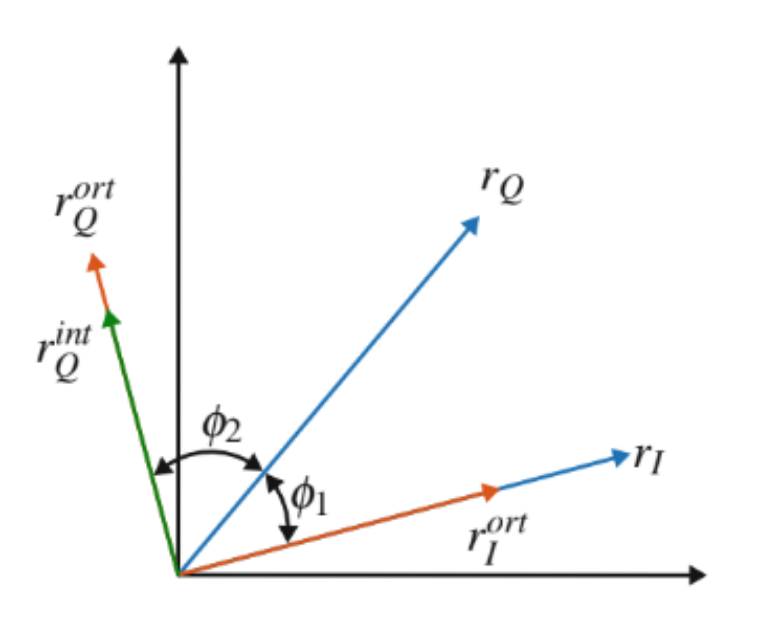
\includegraphics[width=\linewidth]{Ortogonalizador}
    \caption{}
    \label{fig:gsop-vec}
  \end{subfigure}\hfill
  \begin{subfigure}[b]{0.60\linewidth}
    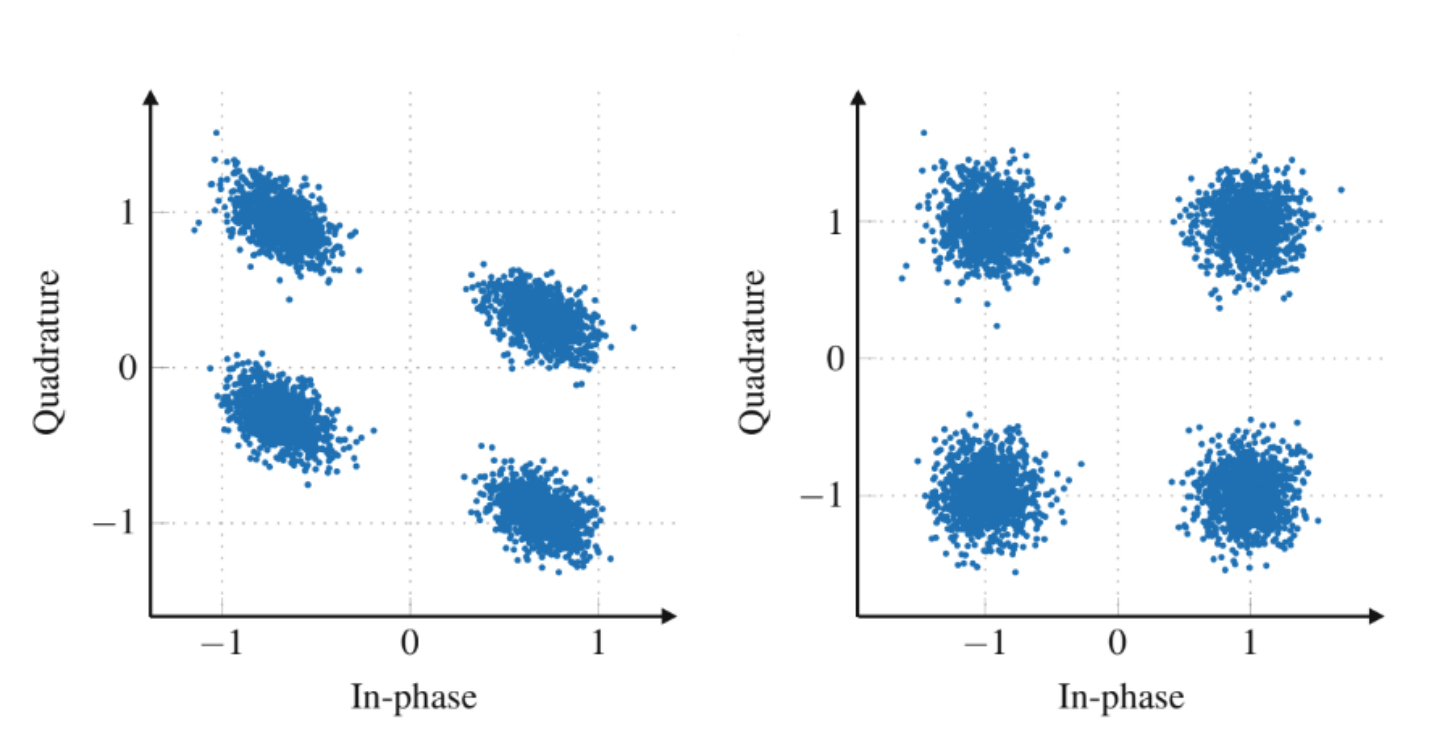
\includegraphics[width=\linewidth]{OrtogonalizadorAntesYDespues}
    \caption{}
    \label{fig:gsop-const}
  \end{subfigure}
  \caption[Ortogonalizaci\'on de Gram--Schmidt]{%
    (a) Construcci\'on: $r_I$ se conserva como referencia y a $r_Q$ se le resta
    su proyecci\'on sobre $r_I$, de modo que $r_Q^{\mathrm{ort}}$ queda
    perpendicular a $r_I^{\mathrm{ort}}$. Los \'angulos $\phi_1$ y $\phi_2$ son
    los que separan a cada carril de su posici\'on ideal. (b) Constelaci\'on
    antes y despu\'es: las nubes inclinadas y el rombo se convierten en nubes circulares.}
  \label{fig:gsop}
\end{figure}

La \cref{fig:gsop} muestra un ejemplo del procedimiento aplicado sobre una
se\~nal QPSK. En el panel~(a) se ve la construcci\'on geom\'etrica, donde los
\'angulos $\phi_1$ y $\phi_2$ miden cu\'anto se aparta cada carril de su
posici\'on ideal. En el panel~(b) se observa el efecto sobre la
constelaci\'on, donde las nubes inclinadas que forman un rombo pasan a ser
circulares y quedan centradas sobre los cuatro puntos ideales, caracter\'istico del ruido aditivo blanco gaussiano.

El procedimiento supone que la se\~nal ideal cumple $\E{s_I s_Q} = 0$, lo cual
vale para QPSK con s\'imbolos independientes. Corrige el \'angulo de
cuadratura y la ganancia relativa, pero no el skew temporal entre las ramas en
fase y en cuadratura. Ese efecto queda a cargo del ecualizador de la
\cref{sec:dsp-ddlms}, que por ser fraccionado en $T/2$ y tener filtros reales
para cada rama puede, en principio, compensarlo.

\paragraph{Verificaci\'on}
El bloque se puso a prueba realizando un barrido param\'etrico de la ganancia
relativa entre las ramas en fase y en cuadratura de las dos polarizaciones,
desde la condici\'on balanceada hasta un cociente de \num{0.30}. El desbalance
se inyect\'o sobre la fotocorriente, que es donde nace una diferencia de
responsividad entre los pares de fotodiodos balanceados.

\begin{figure}[H]
  \centering
  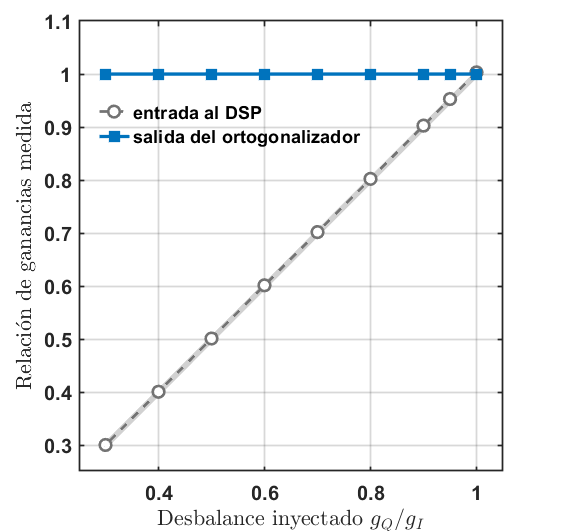
\includegraphics[width=0.6\textwidth]{figuras/DesbalanceGanancias.png}
  \caption[Compensaci\'on del desbalance de ganancia]{%
    Cociente entre la potencia de la rama en cuadratura y la de la rama en
    fase, medido a la entrada del procesamiento y a la salida del
    ortogonalizador, contra el desbalance inyectado.}
  \label{fig:gsop-ganancia}
\end{figure}

La \cref{fig:gsop-ganancia} compara el cociente de potencias a la entrada del
procesamiento y a la salida del ortogonalizador. A la salida vale \num{1.00}
en todo el barrido, y el EVM se mantiene en \SI{31.46}{\percent} en los nueve
puntos. El motivo es que el desbalance se aplica despu\'es de la
fotodetecci\'on y todo lo que sigue hasta el ortogonalizador es lineal, de
modo que el factor llega intacto a la normalizaci\'on y all\'i se cancela. La
medici\'on se hizo con el ruido del preamplificador, que es el dominante del
enlace, y ese ruido lo escalan los fotodetectores igual que a la se\~nal
\'optica, por lo que la relaci\'on se\~nal-ruido no cambia.

Seguidamente se gener\'o un error de desbalance de cuadratura de \ang{10}
junto con el de ganancia, para verificar que el algoritmo es capaz de
estimarlo. El ortogonalizador devuelve \ang{10.26} para todos los valores de
ganancia, lo que verifica la \cref{eq:gsop-phi}.

\section{Recuperaci\'on de frecuencia}
\label{sec:dsp-frec}

Como se describi\'o en la \cref{sec:canal-doppler}, el enlace LEO--GEO impone
un corrimiento Doppler de hasta \SI{4.94}{\giga\hertz} sobre la portadora, al
que se suma la incerteza absoluta de los dos l\'aseres. Por esa raz\'on
resulta necesario estudiar los l\'imites de este bloque.

\paragraph{Prop\'osito}
Compensa la diferencia de frecuencia $\Df$ entre el l\'aser transmisor y el
oscilador local, que en banda base aparece como una rotaci\'on continua de la
constelaci\'on a raz\'on de $2\pi\Df$ radianes por segundo.

\paragraph{Principio de operaci\'on}
Se implement\'o el algoritmo de cuarta potencia, que estima el offset en el
dominio de la frecuencia a partir del espectro de la se\~nal elevada a la
cuarta potencia~\cite[ec.~(6.4)]{mello2021}. La \cref{fig:foc-diagrama} muestra 
la estructura del bloque, donde se ve que
la estimaci\'on se calcula sobre un bloque de muestras y se aplica luego a la
se\~nal completa, sin realimentaci\'on.

Para explicar su funcionamiento, cons\'iderese que la se\~nal compleja
adquirida, en presencia de un offset de frecuencia $\Df$ y en ausencia de
ruido e interferencia entre s\'imbolos, puede escribirse como
\begin{equation}
  y[k] = A\, e^{\,j\left(2\pi\Df\,k/F_s + \theta_0\right)}\,
         e^{\,j\varphi_k}, \qquad
         \varphi_k \in \left\{\tfrac{\pi}{4}, \tfrac{3\pi}{4},
                              \tfrac{5\pi}{4}, \tfrac{7\pi}{4}\right\},
  \label{eq:foc-senal}
\end{equation}
donde $k$ recorre las muestras a la tasa del conversor, $F_s = 2\Rs$, y
$\varphi_k$ es la fase del s\'imbolo QPSK.

Para estimar y posteriormente compensar el valor de $\Df$ se utiliza una propiedad de
QPSK. Las cuatro fases posibles de la modulaci\'on est\'an separadas por
$\pi/2$, as\'i que al elevar a la cuarta potencia
\begin{equation}
  y^4[k] = A^4\, e^{\,j\left(8\pi\Df\,k/F_s + 4\theta_0\right)}\,
           \underbrace{e^{\,j 4\varphi_k}}_{=\,-1\ \forall k},
  \label{eq:foc-cuarta}
\end{equation}
la dependencia con el dato desaparece y lo que queda es una sinusoide pura de
frecuencia $4\Df$. El estimador la ubica computando el valor m\'aximo de la
transformada de Fourier de una secuencia de muestras y divide por cuatro,
\begin{equation}
  \widehat{\Df} = \frac{1}{4}\,
    \arg\max_{f}\ \abs{\mathcal{F}\{y^4[k]\}}.
  \label{eq:foc-estimador}
\end{equation}
La correcci\'on consiste en multiplicar la se\~nal por
$e^{-j2\pi\widehat{\Df}k/F_s}$.

\begin{figure}[H]
  \centering
  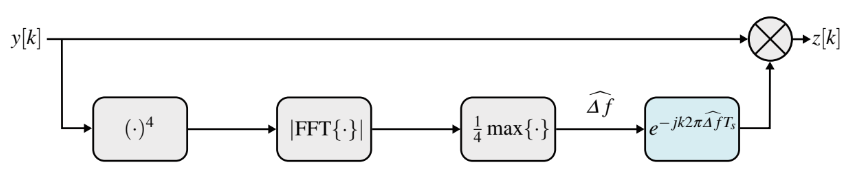
\includegraphics[width=0.86\linewidth]{FRecovery1}
  \caption[Estimador de frecuencia de cuarta potencia]{%
    Estructura del estimador. La rama inferior calcula
    $\widehat{\Df}$ sobre un bloque de muestras y la superior aplica la
    correcci\'on a la se\~nal completa. Es una estimaci\'on de lazo abierto.}
  \label{fig:foc-diagrama}
\end{figure}

\begin{figure}[H]
  \centering
  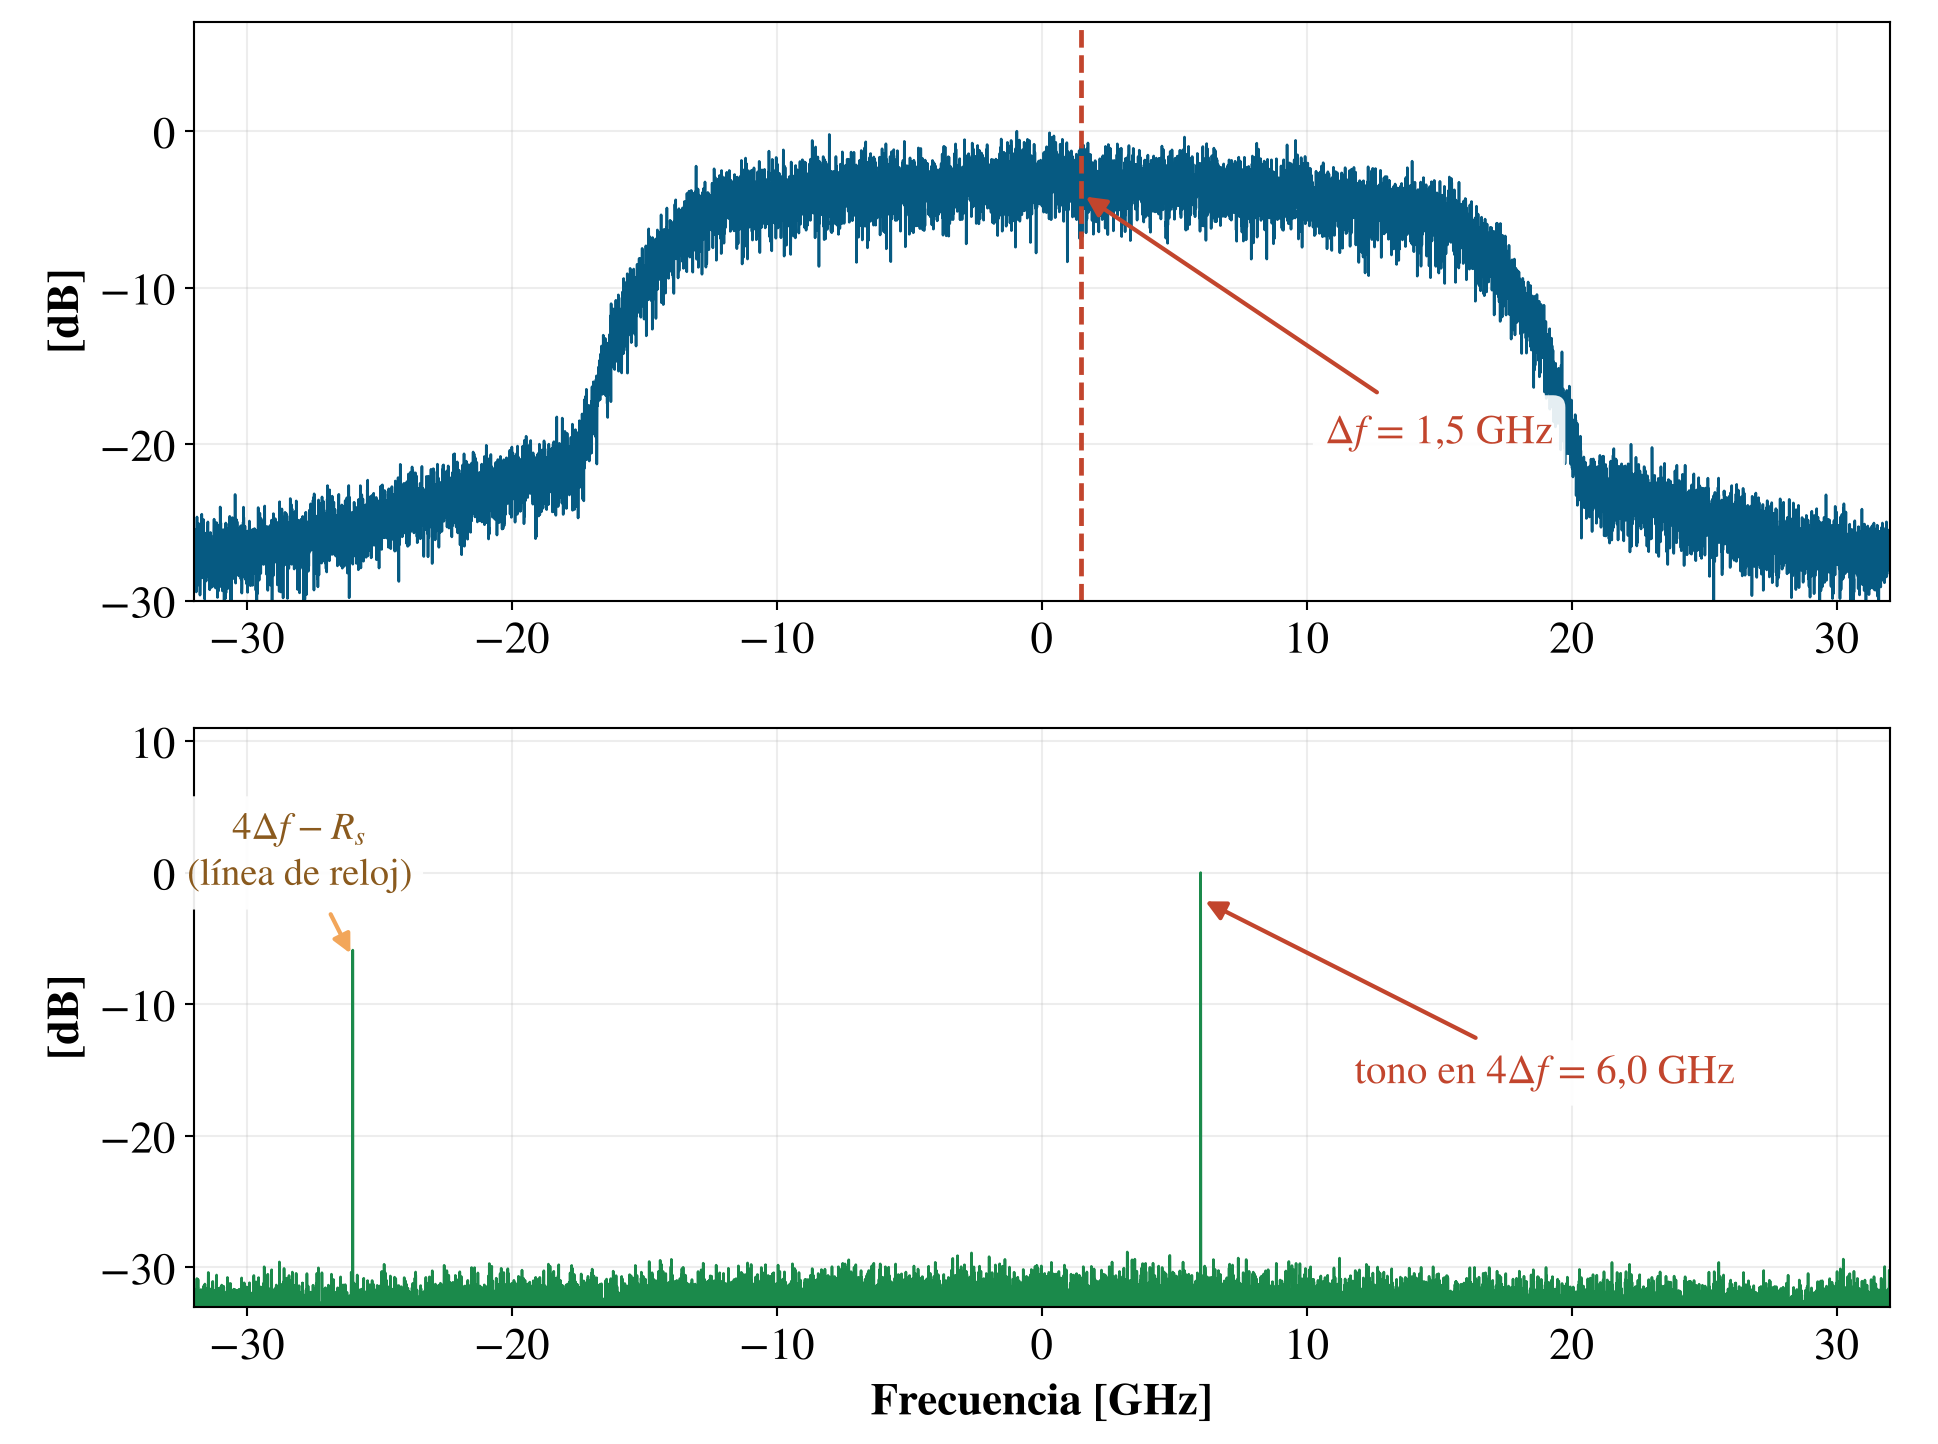
\includegraphics[width=0.9\linewidth]{fourth_power}
  \caption[Espectro antes y despu\'es de elevar a la cuarta potencia]{%
    Simulaci\'on a \SI{32}{\giga\baud} con $\Df = \SI{1.5}{\giga\hertz}$ y
    $\OSNR$ de \SI{16}{\dB}. La imagen superior muestra el espectro de $y[k]$. La inferior muestra c\'omo, elevando a la cuarta potencia, aparece una l\'inea espectral de
    m\'as de \SI{20}{\dB} sobre el piso, exactamente en
    $4\Df = \SI{6}{\giga\hertz}$. La l\'inea de reloj, \SI{6}{\dB} m\'as abajo, est\'a
    en $4\Df - \Rs$.}
  \label{fig:foc-espectro}
\end{figure}

La \cref{fig:foc-espectro} ilustra las
dos etapas del algoritmo sobre el espectro de una simulaci\'on. En el panel
superior, el espectro de $y[k]$ no presenta ninguna l\'inea discreta, porque
la modulaci\'on distribuye la energ\'ia sobre toda la banda. En el inferior, tras
elevar a la cuarta potencia, aparece un tono que sobresale m\'as de
\SI{20}{\dB} del piso y se ubica exactamente en $4\Df$, que es lo que el
estimador busca. Se distingue adem\'as una segunda l\'inea, \SI{6}{\dB} por
debajo y separada $\Rs$ de la principal, cuyo origen y consecuencias se
analizan en la \cref{sec:dsp-frec-limite}.

\subsection{L\'imite de captura}
\label{sec:dsp-frec-limite}

Tres mecanismos distintos pueden limitar el rango de offset que el estimador
resuelve correctamente.

\paragraph{(A) Plegado de Nyquist del tono de cuarta potencia:}
Al elevar a la cuarta potencia, el tono derivado del offset de frecuencia se
encuentra en $4\Df$. Como la se\~nal est\'a muestreada a $F_s = 2\Rs$, la
transformada solo representa frecuencias entre $-F_s/2$ y $+F_s/2$. Si
$4\abs{\Df}$ supera $F_s/2$, el tono cae fuera de ese rango y reaparece
plegado por el borde opuesto, donde el estimador lo toma como v\'alido. De
modo que el m\'aximo offset de frecuencia tolerado para que el estimador
funcione sin ambig\"uedad es
\begin{equation}
  \abs{\Df} < \frac{F_s}{8} = \frac{\Rs}{4} = \SI{8}{\giga\hertz}
  \qquad (\text{a } \Rs = \SI{32}{\giga\baud}).
  \label{eq:limite-nyquist}
\end{equation}

\begin{figure}[H]
  \centering
  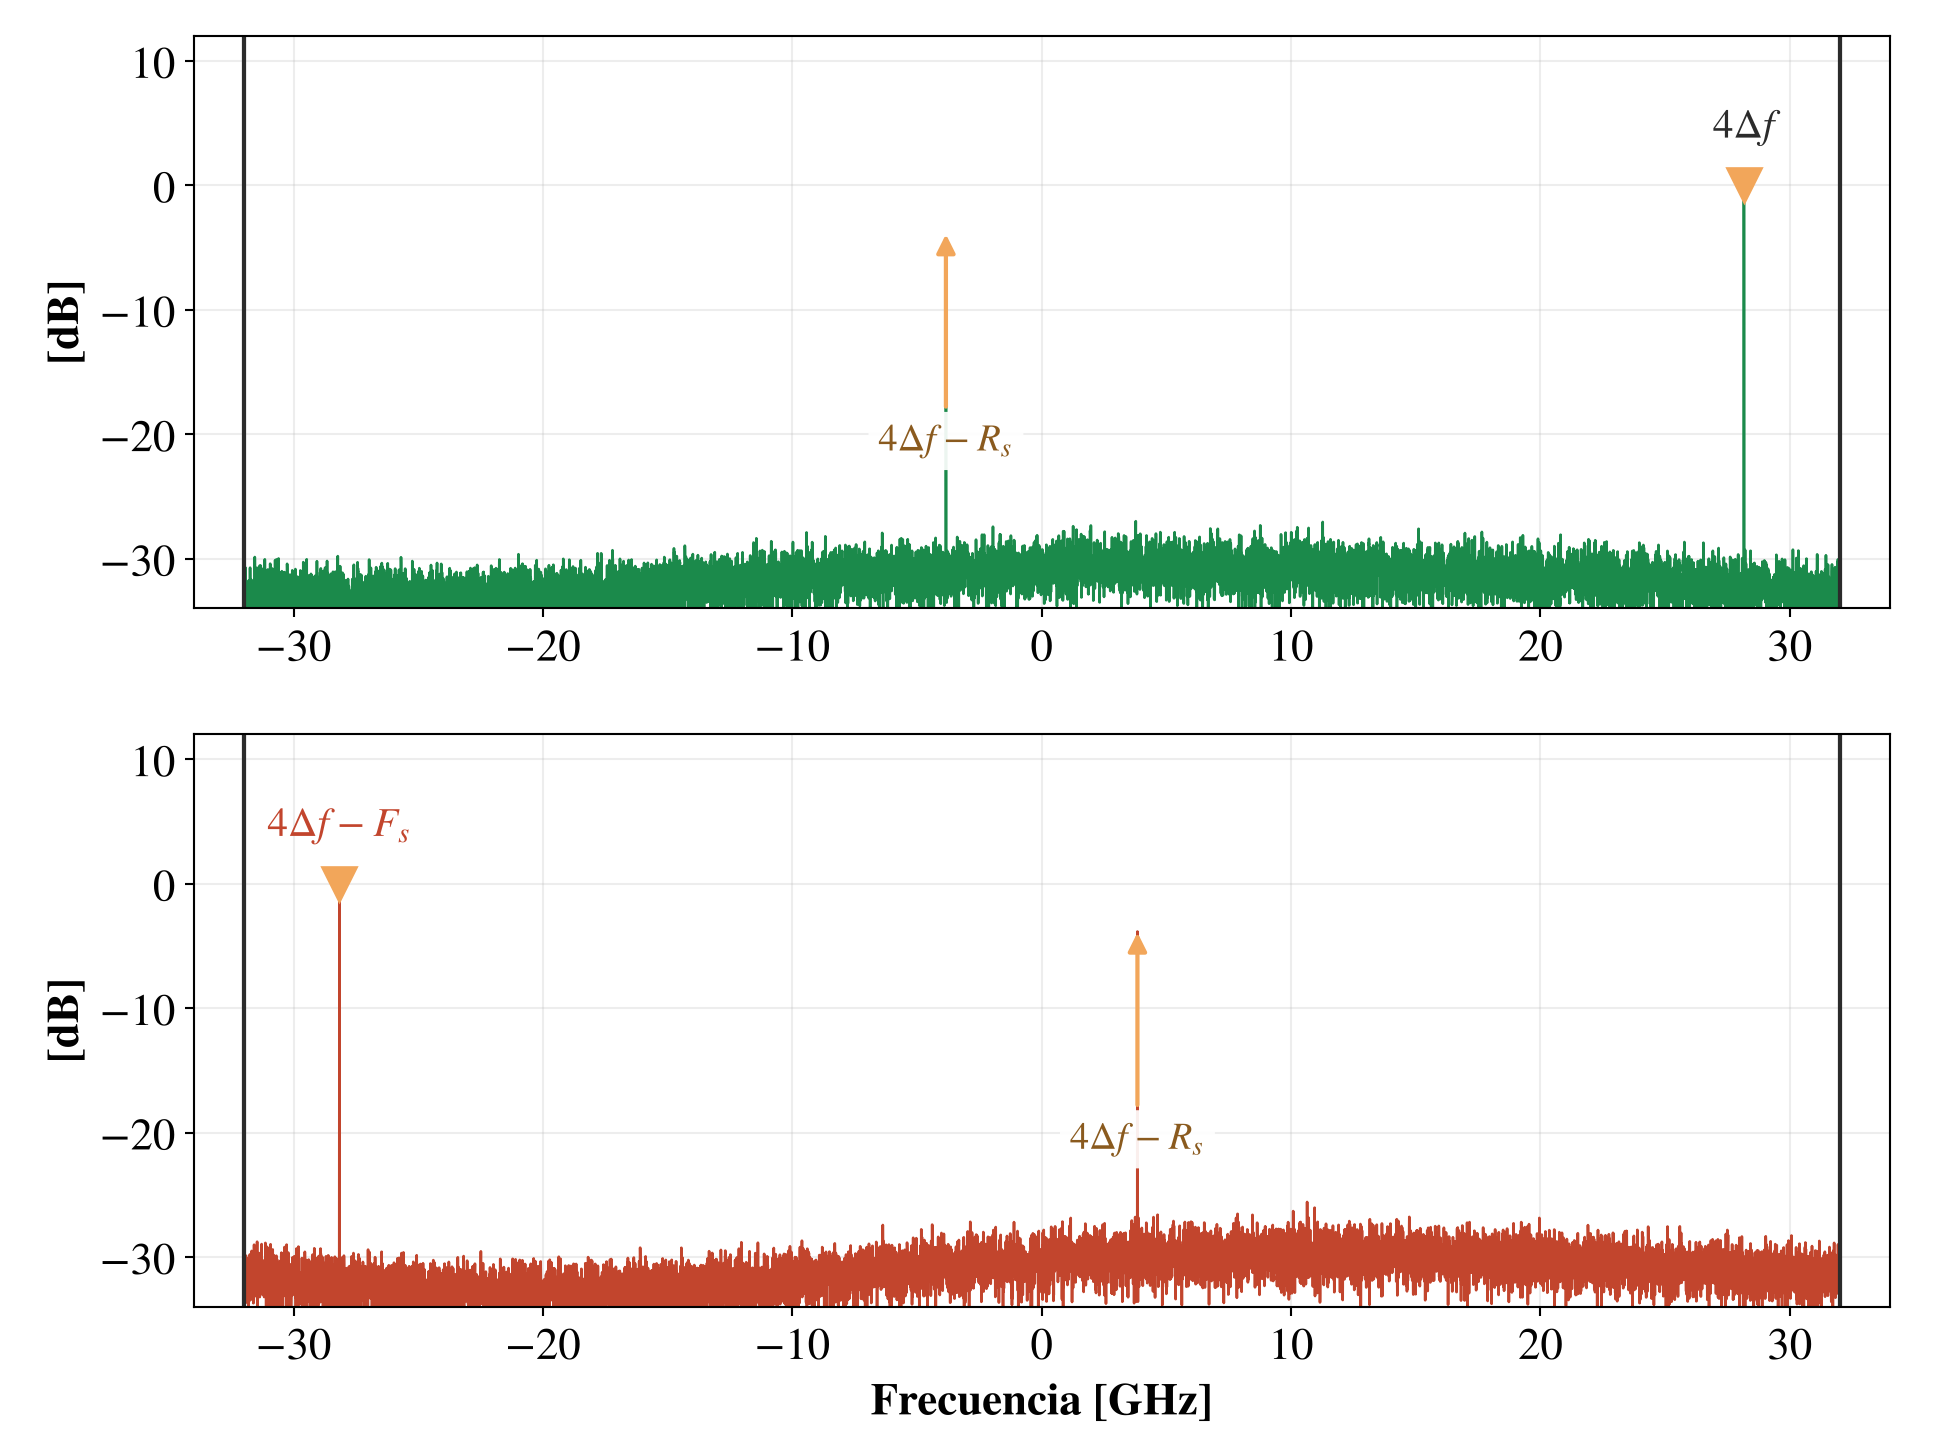
\includegraphics[width=0.9\linewidth]{limite_captura}
  \caption[Techo de captura por plegado de Nyquist]{%
    Espectro de $y^4[k]$ a los dos lados del techo~(A). Arriba, con
    $\Df = 0{,}22\,\Rs$ el tono de cuarta potencia cae dentro de la banda y la
    estimaci\'on es exacta. Abajo, con $\Df = 0{,}28\,\Rs$ el tono deber\'ia
    estar en \SI{35.84}{\giga\hertz}, fuera de $\pm F_s/2$. Sin embargo, reaparece plegado en
    \SI{-28.16}{\giga\hertz} y el estimador devuelve \SI{-7.04}{\giga\hertz} en
    lugar de \SI{8.96}{\giga\hertz}, un salto de $-\Rs/2$. En los dos paneles se
    ve tambi\'en la l\'inea de reloj en $4\Df - \Rs$, que en el panel de abajo ya
    est\'a a \SI{3.7}{\dB} del pico.}
  \label{fig:foc-limite}
\end{figure}

La \cref{fig:foc-limite} muestra un ejemplo de lo que ocurre a los dos lados
del umbral. En el panel superior, con $\Df = 0{,}22\,\Rs$, el tono de
cuarta potencia cae dentro de la banda representable y la estimaci\'on
coincide con el valor inyectado. En el inferior, con $\Df = 0{,}28\,\Rs$, el
tono deber\'ia ubicarse en \SI{35.84}{\giga\hertz}, por encima de $F_s/2$. Se
puede observar c\'omo reaparece en \SI{-28.16}{\giga\hertz}, de donde el
estimador devuelve \SI{-7.04}{\giga\hertz} en lugar de
\SI{8.96}{\giga\hertz}. El salto es de $-\Rs/2$ y ocurre sin degradaci\'on
previa, porque no se trata de una p\'erdida de precisi\'on sino de una
ambig\"uedad del rango representable.

\paragraph{(B) L\'inea de reloj:}
La ciclo\-estacionariedad del pulso conformado genera adem\'as l\'ineas
espectrales en $4\Df \pm k\Rs$. A medida que el offset
crece, el tono principal se acerca al borde de la banda del receptor, donde el
front end de \SI{20}{\giga\hertz} y el conversor de \SI{33}{\giga\hertz} lo
aten\'uan, mientras que la l\'inea ubicada $\Rs$ m\'as abajo queda en una zona
menos atenuada. Si llegara a superar al tono principal, la estimaci\'on
tendr\'ia un salto de  $-\Rs/4$, distinto al que produce el plegado y por lo
tanto reconocible.

El mecanismo se observa en las dos figuras anteriores. Con
$\Df = \SI{1.5}{\giga\hertz}$ la l\'inea de reloj est\'a \SI{6}{\dB} por
debajo del tono principal, y con el offset mayor de la \cref{fig:foc-limite}
esa distancia ya se redujo a \SI{3.7}{\dB}. En ninguna de las condiciones
ensayadas con $\beta = 0{,}2$ lleg\'o a predominar antes de alcanzarse el
l\'imite~(A).

\paragraph{(C) Ancho de banda de adquisici\'on:}
Este l\'imite no es debido al estimador sino al muestreo, y se dedujo en la
\cref{sec:trx-nyquist}. La se\~nal llega centrada en $\Df$ y ocupa
$[\Df - B,\ \Df + B]$, con $B = (1+\beta)\Rs/2$, de manera que para no
plegarse tiene que entrar por completo en la banda del
conversor,
\begin{equation}
  \abs{\Df} \leq \frac{F_s}{2} - B .
  \label{eq:limite-adc}
\end{equation}
Con $F_s = 2\Rs = \SI{64}{\giga\hertz}$ y $B = \SI{19.2}{\giga\hertz}$ el
l\'imite vale \SI{12.8}{\giga\hertz}, holgadamente por encima del techo~(A).


\paragraph{Conclusi\'on}
El mecanismo que predomina en la cadena simulada es el~(A). No se trata de una
degradaci\'on progresiva ni de una cuesti\'on de relaci\'on se\~nal-ruido,
sino del rango de la funci\'on que implementa el estimador, que busca un
m\'aximo sobre un eje de frecuencias acotado a $\pm F_s/2$. Para $\Rs = \SI{32}{\giga\baud}$,
\begin{equation}
  \abs{\widehat{\Df}} \leq \frac{\Rs}{4} = \SI{8}{\giga\hertz}.
  \label{eq:techo-duro}
\end{equation}

El requerimiento del enlace, establecido en el \cref{cap:canal}, es de
\SI{6.0}{\giga\hertz}, de los cuales \SI{4.94}{\giga\hertz} corresponden al
Doppler y \SI{1}{\giga\hertz} a la incerteza combinada de los dos l\'aseres.
Contra el l\'imite de \SI{8}{\giga\hertz} queda un \SI{33}{\percent} de margen.

El rango de captura escala \'unicamente con $\Rs$, de modo que bajar la tasa
de s\'imbolo lo reduce en la misma proporci\'on. El \cref{cap:tolerancias}
verifica estos l\'imites sobre un barrido de offset, y analiza en qu\'e medida
la relaci\'on se\~nal-ruido y el ancho de banda del receptor los modifican.

\section{Filtro adaptado y recuperaci\'on de reloj}
\label{sec:dsp-mf-clock}

\subsection{Filtro adaptado}
\label{sec:dsp-mf}

\paragraph{Prop\'osito}
Maximiza la relaci\'on se\~nal-ruido en el instante de decisi\'on y, junto con
la conformaci\'on de pulso del transmisor, completa el par que en principio
cumple el criterio de Nyquist.

\paragraph{Principio de operaci\'on}
Se trata del mismo RRC del transmisor, con $\beta = 0{,}2$, implementado como filtro
FIR a la tasa del conversor.

\begin{figure}[H]
  \centering
  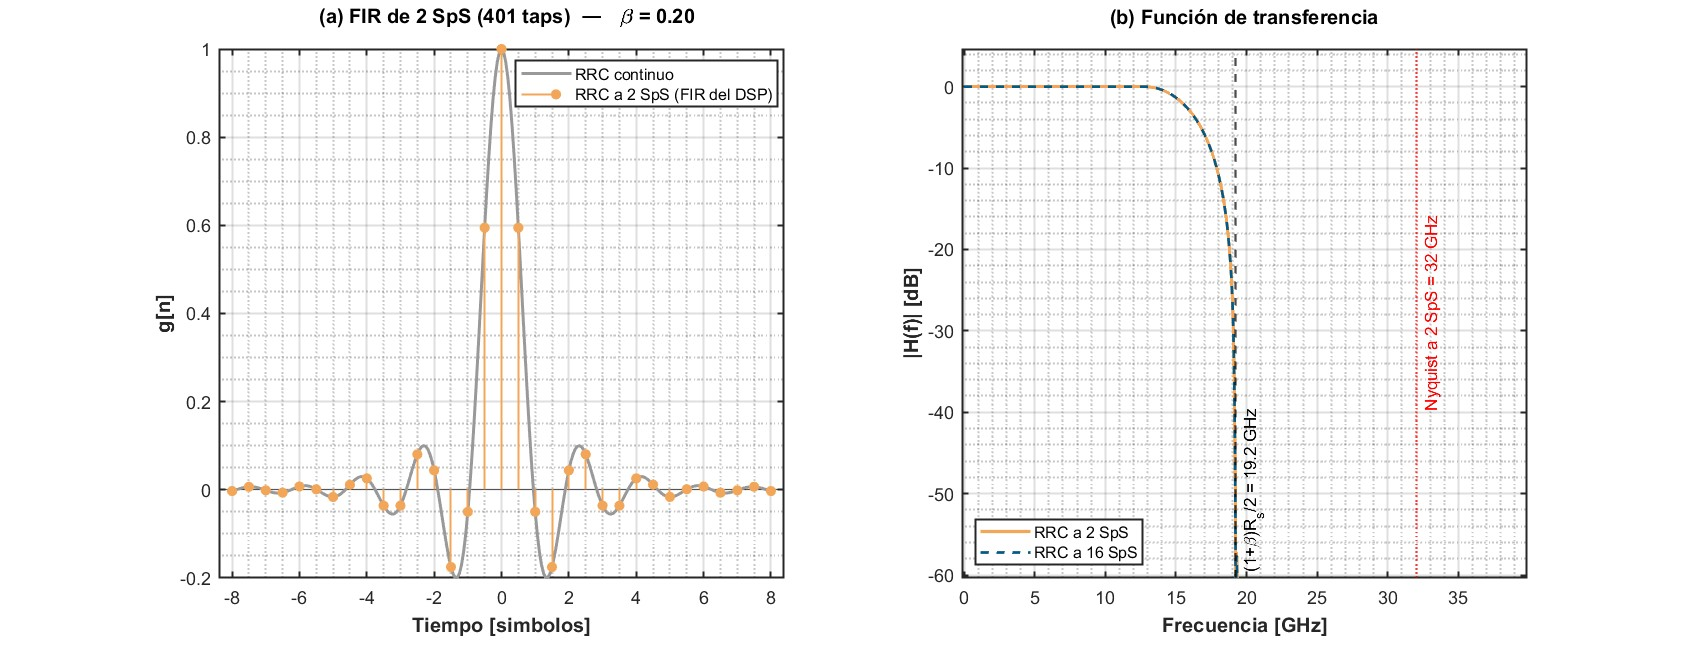
\includegraphics[width=0.95\linewidth]{FiltroFIRdelDSP}
  \caption[Filtro adaptado del receptor]{%
    (a) Respuesta al impulso: los \num{401} coeficientes del FIR caen
    exactamente sobre el RRC continuo. (b) Funci\'on de transferencia: la versi\'on a
    \num{2} muestras por s\'imbolo coincide con la de \num{16} hasta muy por debajo de
    $(1+\beta)\Rs/2 = \SI{19.2}{\giga\hertz}$, y el borde de Nyquist a \num{2}
    muestras por s\'imbolo, que est\'a en \SI{32}{\giga\hertz}, queda holgadamente por encima.}
  \label{fig:fir}
\end{figure}

La \cref{fig:fir} verifica que implementarlo a dos muestras por s\'imbolo no
altera su respuesta en la banda de inter\'es. En el panel~(a) se observa que
los \num{401} coeficientes del FIR caen sobre la respuesta del RRC continuo.
En el panel~(b) se compara la funci\'on de transferencia a dos y a dieciséis
muestras por s\'imbolo, y las dos coinciden hasta bastante m\'as all\'a del
borde de la se\~nal. El borde de Nyquist a dos muestras por s\'imbolo queda en
\SI{32}{\giga\hertz}, holgadamente por encima de los
\SI{19.2}{\giga\hertz} que la se\~nal ocupa.

Cabe resaltar que la cadena completa no cumple el criterio de Nyquist. Entre
los dos filtros RRC se interpone la respuesta del front end de
\SI{20}{\giga\hertz} y la del conversor de \SI{33}{\giga\hertz}, que recortan
el pulso y dejan interferencia entre s\'imbolos residual. Esa es una de las
razones por las que el ecualizador adaptativo de la \cref{sec:dsp-ddlms}
resulta necesario aun sin considerar los deterioros del canal.

\subsection{Lazo de recuperaci\'on de reloj}
\label{sec:dsp-clock}

\paragraph{Prop\'osito}
Por otro lado, la recuperaci\'on de reloj corrige el error de fase de muestreo
que aparece porque el conversor del receptor no est\'a sincronizado con el
reloj del transmisor. A esto se suma el desv\'io de la tasa de s\'imbolo de
\SI{25.55}{\ppm} que introduce el Doppler (\cref{sec:canal-doppler}).

\paragraph{Principio de operaci\'on}
El bloque reconstruye el valor que la se\~nal habr\'ia tenido en el instante
de muestreo correcto, interpolando entre las muestras disponibles. El instante
lo fija un lazo cerrado.

\begin{figure}[H]
  \centering
  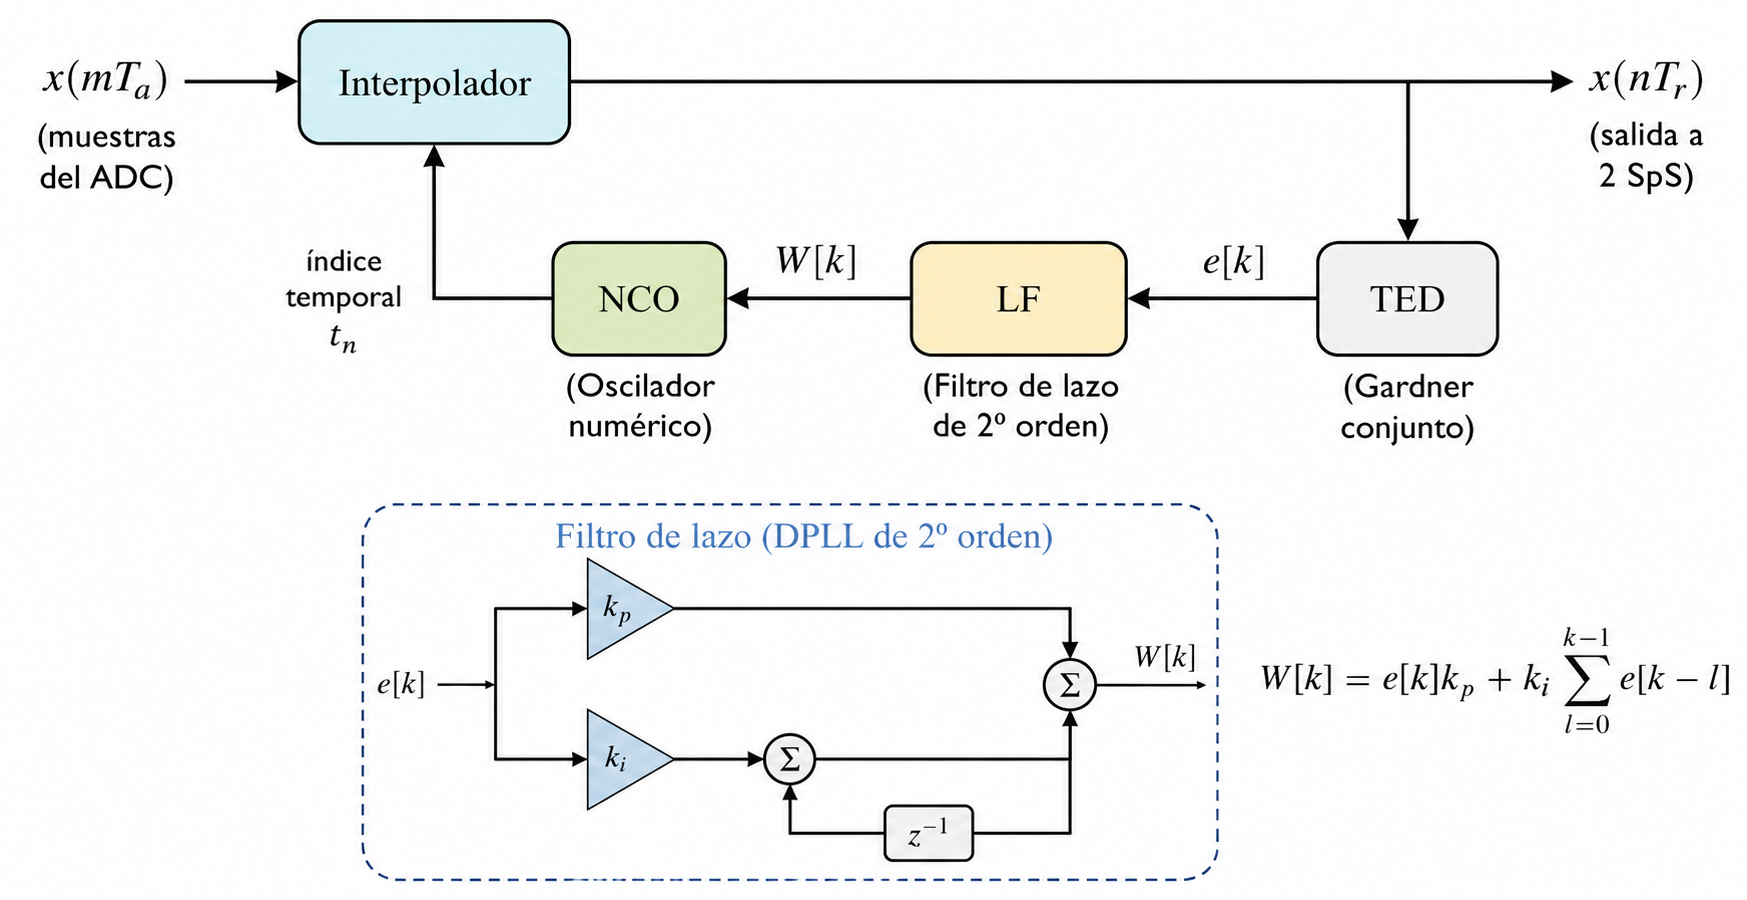
\includegraphics[width=\linewidth]{ClockRecoveryDiagrama2}
  \caption[Lazo de recuperaci\'on de reloj]{%
    Recuperaci\'on de reloj: interpolador controlado por un lazo cerrado. El
    detector de error de tiempo (TED) mide cu\'anto se aparta el instante de
    muestreo del \'optimo, el filtro de lazo PI integra el error y el
    oscilador num\'erico (NCO) produce el \'indice temporal $t_n$ con el que el
    interpolador reconstruye la muestra. Abajo, el filtro de lazo: rama
    proporcional $k_p$, rama integral $k_i$ con su acumulador.}
  \label{fig:clock}
\end{figure}

La \cref{fig:clock} muestra los tres elementos del lazo. El detector de error
de tiempo mide cu\'anto se aparta el instante de muestreo del \'optimo, el
filtro proporcional-integral promedia el error, y el oscilador num\'erico
acumula el resultado para producir el \'indice temporal con el que el
interpolador reconstruye cada muestra.

\paragraph{Detector de error de tiempo}
Se implementa el detector de Gardner~\cite{gardner1986}, que opera a dos muestras por
s\'imbolo. Toma el centro del s\'imbolo actual, el del anterior y la muestra
intermedia, que idealmente cae en el cruce por cero, y calcula
\begin{equation}
  e[k] = \Re\!\left\{\left(x_k - x_{k-1}\right)\, x_{k-1/2}^{*}\right\}.
  \label{eq:gardner}
\end{equation}
Si el muestreo est\'a en el instante \'optimo, el pulso es sim\'etrico
alrededor del cruce, la muestra intermedia cae en cero y el producto se anula.
Si est\'a adelantado o atrasado, la muestra intermedia toma un valor no nulo
cuyo signo indica la direcci\'on del desv\'io. El factor $(x_k - x_{k-1})$
aporta la direcci\'on de la transici\'on, de modo que el signo del error no
dependa de qu\'e s\'imbolos se hayan transmitido. El error se suma sobre las
dos polarizaciones, $e[k] = e_V[k] + e_H[k]$, para que un desvanecimiento en
una de ellas no deje al lazo sin se\~nal.

\paragraph{Interpolador}
La reconstrucci\'on usa un interpolador c\'ubico sobre las cuatro muestras
adyacentes al instante deseado.

\paragraph{Par\'ametros del lazo}
El filtro de lazo es proporcional-integral, as\'i que el conjunto
TED\,--\,filtro\,--\,NCO constituye un lazo de segundo orden, o de tipo~2. Sus
par\'ametros can\'onicos son~\cite[ec.~(7.10)--(7.12)]{mello2021}
\begin{equation}
  \omega_n T = \sqrt{k_i K_d},
  \qquad
  \zeta = \frac{k_p}{2}\sqrt{\frac{K_d}{k_i}},
  \qquad
  B_L = \frac{\omega_n}{2}\left(\zeta + \frac{1}{4\zeta}\right).
  \label{eq:lazo-2do}
\end{equation}
Ac\'a $k_p$ y $k_i$ son las ganancias de las ramas proporcional e integral del
filtro, $K_d$ es la sensibilidad del detector, $T = 1/\Rs$ el per\'iodo de
s\'imbolo, $\omega_n$ la frecuencia natural del lazo, $\zeta$ su factor de
amortiguamiento y $B_L$ su ancho de banda de ruido unilateral. Este \'ultimo
es el que gobierna el compromiso entre seguir variaciones r\'apidas del reloj
y filtrar el ruido.

Combinando las dos primeras expresiones se obtiene $\omega_n\zeta = k_p K_d/(2T)$
y $\omega_n/(4\zeta) = k_i/(2 k_p T)$, de modo que las ra\'ices se cancelan y
el ancho de banda queda en forma cerrada,
\begin{equation}
  B_L = \frac{\Rs}{4}\left( k_p K_d + \frac{k_i}{k_p} \right).
  \label{eq:BL-cerrada}
\end{equation}
La rama proporcional entra multiplicada por la ganancia del detector y la
integral dividida por la proporcional.

La sensibilidad $K_d$ es la pendiente de la curva caracter\'istica del
detector en el origen, que se obtiene de la \cref{tab:gardner-beta} m\'as
adelante. Para $\beta = 0{,}2$ vale \num{0.63}. Con $k_p = \num{e-3}$ y
$k_i = \num{e-7}$ se tiene
\begin{equation}
  f_n = \frac{\omega_n}{2\pi} = \SI{1.28}{\mega\hertz},
  \qquad
  \zeta = \num{1.25},
  \qquad
  B_L = \SI{5.8}{\mega\hertz}.
  \label{eq:lazo-reloj}
\end{equation}
Con $\zeta > 1$ el lazo queda sobreamortiguado, sin sobrepico. Su tiempo de
respuesta, estimado como $1/(2B_L)$, es de \SI{86}{\nano\second}, lo que a
\SI{32}{\giga\baud} se corresponde con unos \num{2750} s\'imbolos.

\paragraph{L\'imites del lazo}
De estos par\'ametros surgen tres consecuencias para el enlace.

\begin{itemize}

\item \textbf{Desv\'io constante de la tasa de muestreo:} Un lazo de tipo~2
sigue una rampa de fase sin dejar error en r\'egimen permanente, de modo que
el desv\'io de \SI{25.55}{\ppm} que impone el Doppler
(\cref{sec:canal-doppler}) queda compensado por completo. Ese desv\'io
equivale a una deriva del instante de muestreo de \SI{8.2e5}{} s\'imbolos por
segundo, que la rama integral alcanza en unos \num{250} s\'imbolos, dentro de
la ventana de entrenamiento del ecualizador.

\item \textbf{Aceleraci\'on:} Lo que un lazo de tipo~2 s\'i deja como error
est\'atico es la variaci\'on del desv\'io. La aceleraci\'on radial del pase,
$a_r = \SI{10.15}{\meter\per\second\squared}$, hace variar la tasa a raz\'on
de $a_r/c = \SI{3.4e-8}{\per\second}$, lo que en el instante de muestreo
representa una aceleraci\'on de \num{1083} s\'imbolos por segundo al cuadrado.
El error residual que deja es
\begin{equation}
  \tau_{ss} = \frac{\ddot\tau}{\omega_n^2}
            = \SI{1.7e-11}{}\ \text{s\'imbolos},
  \label{eq:error-acel}
\end{equation}
despreciable frente al per\'iodo de s\'imbolo.

\item \textbf{Deslizamiento de s\'imbolo:} La curva caracter\'istica del
detector no tiene un \'unico cero, y de ah\'i surge el tercer l\'imite.

\begin{figure}[H]
  \centering
  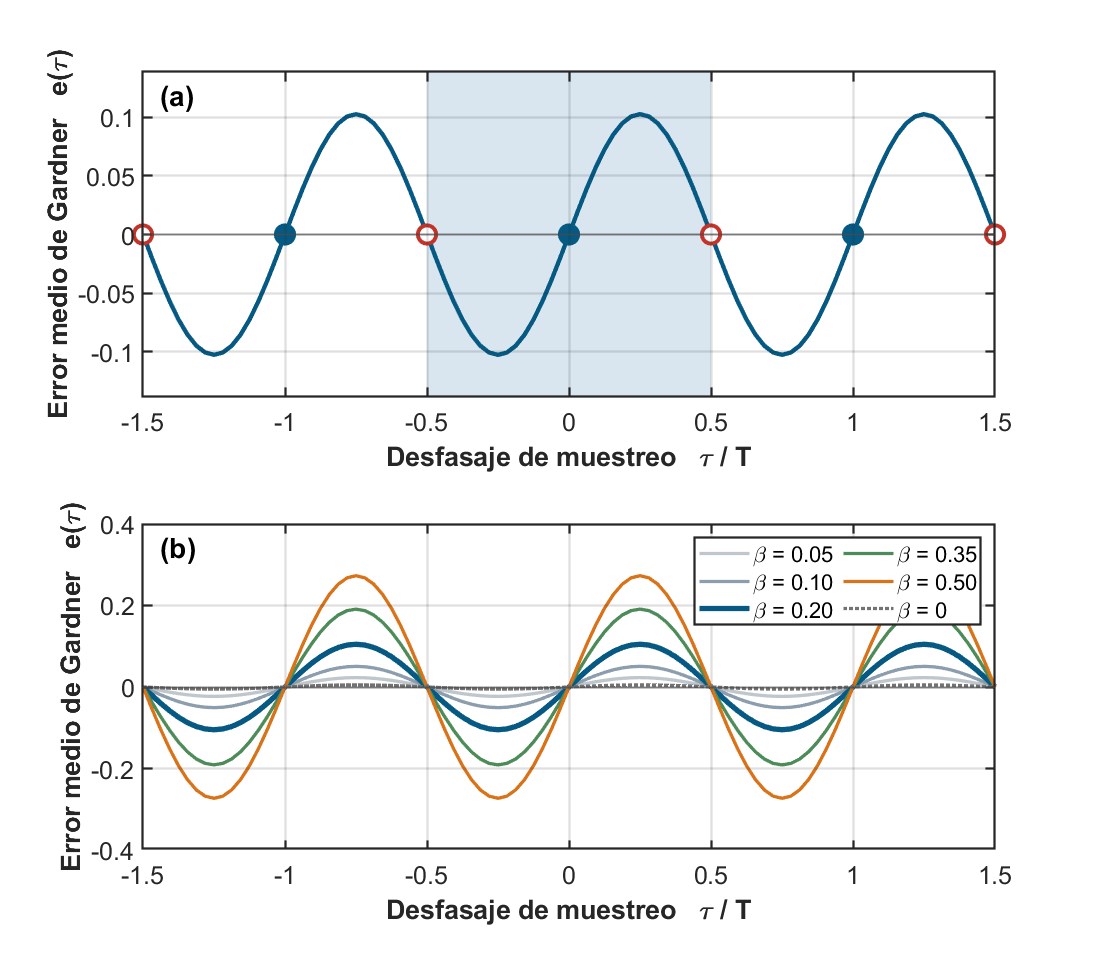
\includegraphics[width=0.92\linewidth]{gardner_scurve}
  \caption[Curva caracter\'istica del detector de Gardner]{%
    Error medio del detector de Gardner en funci\'on del desfasaje de muestreo
    $\tau$, obtenido promediando la \cref{eq:gardner} sobre \num{2e4}
    s\'imbolos QPSK conformados con el par RRC transmisor--receptor.
    \textbf{(a)} Con $\beta = 0{,}2$: la curva completa un ciclo por s\'imbolo.
    Los c\'irculos llenos marcan los puntos de enganche, separados $T$ entre
    s\'i, y los vac\'ios, los cruces intermedios, donde el error tambi\'en se
    anula pero el lazo es inestable. La franja sombreada tiene ancho $T$ y es
    el intervalo de captura alrededor de un punto de enganche.
    \textbf{(b)} El mismo barrido para varios \emph{roll-off}. La amplitud, y
    con ella la pendiente en el origen, se reducen a cero al disminuir $\beta$.}
  \label{fig:gardner-scurve}
\end{figure}

La \cref{fig:gardner-scurve} muestra el error medio del detector en funci\'on
del desfasaje de muestreo. Como se ve en el panel~(a), la curva es
peri\'odica con per\'iodo $T = 1/\Rs = \SI{31.25}{\pico\second}$, es decir que
el detector completa un ciclo entero por cada s\'imbolo que se corre el
instante de muestreo.

La consecuencia es que el punto de enganche no es \'unico. El error se anula
cada $T/2$, alternando el signo de la pendiente. Los cruces con pendiente de
un signo son puntos de equilibrio estable, porque ante una perturbaci\'on el
error realimentado empuja al lazo de vuelta hacia ellos, y los intermedios son
inestables por la raz\'on opuesta. Los estables est\'an separados $T$ entre
s\'i y el detector entrega el mismo error en todos, de modo que el lazo no
dispone de informaci\'on para distinguirlos. Son todos v\'alidos y difieren en
un s\'imbolo entero.

Eso define un intervalo de captura de $\pm T/2$ alrededor de cada punto de
enganche, que es el \'area sombreada de la figura. Si una perturbaci\'on
desplaza al lazo m\'as all\'a de esa franja antes de que alcance a corregirla,
el lazo converge al punto de enganche vecino y la salida queda corrida un
s\'imbolo entero. Cu\'an r\'apido puede el lazo absorber esa perturbaci\'on lo
determina $B_L$.

\item \textbf{Dependencia con el \emph{roll-off}.} La sensibilidad del
detector depende del conformado del pulso. La informaci\'on de temporizado de
una se\~nal modulada linealmente no est\'a en su espectro de potencia sino en
la correlaci\'on entre componentes separadas $\Rs$, y con un RRC esa
correlaci\'on solo existe en la banda de transici\'on del filtro, de ancho
$\beta\Rs$ a cada lado~\cite{franks1980}. Con $\beta = 0{,}2$ son
\SI{6.4}{\giga\hertz} de cada lado. Al reducir el \emph{roll-off} esa banda se
angosta, hasta que en $\beta = 0$ desaparece y no queda informaci\'on de
temporizado.

\begin{table}[htbp]
  \centering
  \begin{tabular}{ccc}
    \toprule
    $\beta$ & $\abs{K_d}$ & respecto de $\beta = 0{,}2$ \\
    \midrule
    \num{0}    & \num{0.029} & \SI{5}{\percent} \\
    \num{0.05} & \num{0.148} & \SI{24}{\percent} \\
    \num{0.10} & \num{0.337} & \SI{54}{\percent} \\
    \num{0.20} & \num{0.628} & \SI{100}{\percent} \\
    \num{0.35} & \num{1.177} & \SI{187}{\percent} \\
    \num{0.50} & \num{1.746} & \SI{278}{\percent} \\
    \bottomrule
  \end{tabular}
  \caption[Ganancia del detector de Gardner contra el \emph{roll-off}]{%
           Ganancia del detector de Gardner contra el \emph{roll-off},
           medida como la pendiente de la curva S en el origen.}
  \label{tab:gardner-beta}
\end{table}

La \cref{tab:gardner-beta} cuantifica esa dependencia. $K_d$ crece de manera
aproximadamente proporcional a $\beta$, y en $\beta = 0$ la pendiente es dos
\'ordenes de magnitud menor que en el valor adoptado. Seg\'un la
\cref{eq:lazo-2do}, $\omega_n$ y $\zeta$ escalan con $\sqrt{K_d}$, de modo que
bajar el \emph{roll-off} vuelve al lazo m\'as lento y peor amortiguado. Esta
es una de las razones por las que no se redujo $\beta$ por debajo de
\num{0.2}.

\end{itemize}


\section{Ecualizaci\'on adaptativa MIMO}
\label{sec:dsp-ddlms}

\paragraph{Prop\'osito}
Esta funci\'on se encarga de compensar la mezcla din\'amica de las dos
polarizaciones que introduce la rotaci\'on del estado de polarizaci\'on a lo
largo del enlace, la interferencia entre s\'imbolos residual y el skew
temporal entre ramas.

\paragraph{Principio de operaci\'on}
El ecualizador es una estructura mariposa $2\times2$. Cada salida es la suma
de dos filtros FIR aplicados a las dos entradas,
\begin{equation}
  \begin{bmatrix} y_X[k] \\ y_Y[k] \end{bmatrix}
  =
  \begin{bmatrix} \mathbf{h}_{XX} & \mathbf{h}_{XY} \\
                  \mathbf{h}_{YX} & \mathbf{h}_{YY} \end{bmatrix}
  \begin{bmatrix} \mathbf{x}_X[k] \\ \mathbf{x}_Y[k] \end{bmatrix},
  \label{eq:mariposa}
\end{equation}
con \num{7} coeficientes por rama y espaciado fraccionado $T/2$. La entrada
llega a dos muestras por s\'imbolo y la salida se entrega a una. Ese espaciado
fraccionado es lo que le permite corregir retardos de una fracci\'on de
s\'imbolo, es decir el skew.

\begin{figure}[H]
  \centering
  \makebox[\linewidth][c]{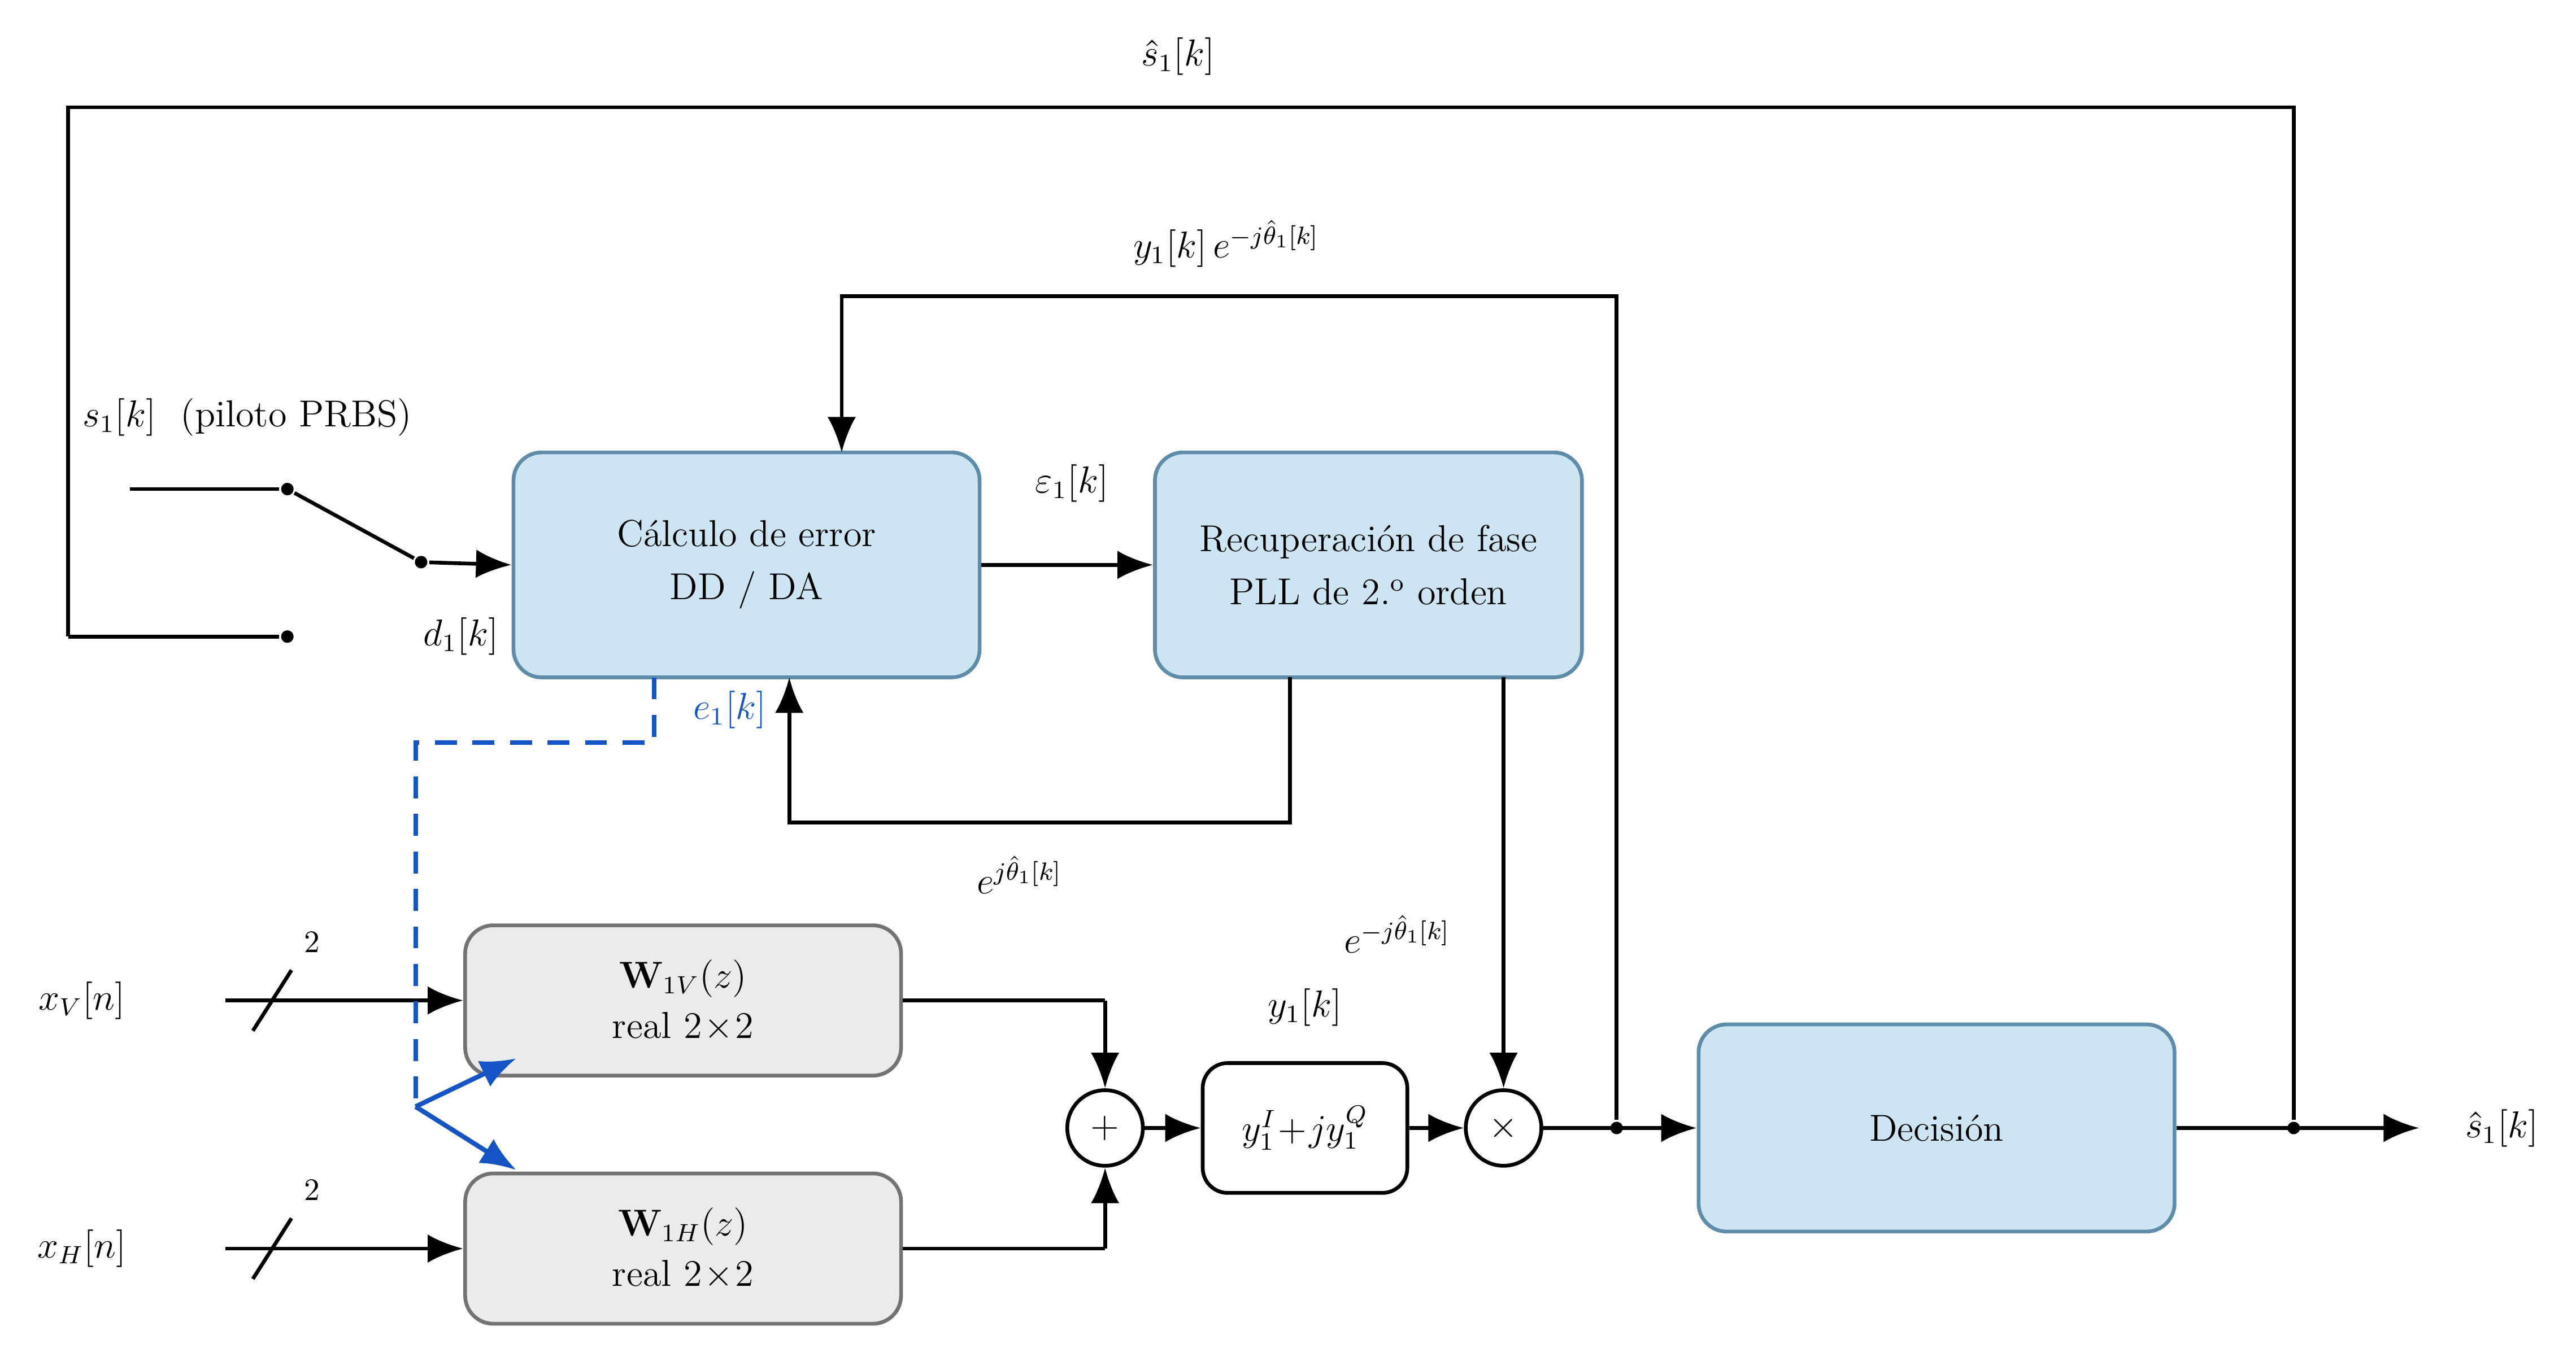
\includegraphics[width=1.12\linewidth]{ddlms_real_pol1_3}}
  \caption[Ecualizador mariposa y lazo de fase]{%
    Rama del ecualizador que genera la polarizaci\'on~V. Las dos entradas
    $x_V[n]$ y $x_H[n]$ llegan a \num{2} muestras por s\'imbolo, cada una pasa
    por su matriz real de $2\times2$ y las dos salidas se suman para formar
    $y_1[k]$ a una muestra por s\'imbolo. El conmutador de arriba a la
    izquierda selecciona la referencia del error: el piloto PRBS durante los
    primeros $N_{\mathrm{tr}}$ s\'imbolos y la propia decisi\'on despu\'es. La
    estructura es sim\'etrica, de modo que la rama que genera la
    polarizaci\'on~H es id\'entica, con sus propias $\mathbf{W}_{2V}$ y
    $\mathbf{W}_{2H}$ y su propio lazo de fase.}
  \label{fig:ddlms}
\end{figure}

La \cref{fig:ddlms} muestra una de las dos ramas de la estructura, la que
genera la polarizaci\'on~V, con el lazo de fase de la \cref{sec:dsp-cpr} ya en
su lugar. La otra rama es id\'entica y opera en paralelo sobre las mismas dos
entradas. En el diagrama se observa c\'omo cada entrada atraviesa su propio
filtro antes de sumarse, y c\'omo el conmutador de la referencia del error
decide si el algoritmo se entrena contra el piloto o contra su propia
decisi\'on.

La regla de actualizaci\'on de los coeficientes del filtro es el gradiente
estoc\'astico del algoritmo LMS~\cite[sec.~5.2]{mello2021},
\begin{equation}
  \mathbf{h}(n+1) = \mathbf{h}(n) + \mu\, e(n)\, \mathbf{x}^{*}(n),
  \label{eq:lms}
\end{equation}
con un paso de adaptaci\'on $\mu = 0{,}01$. El error $e(n)$ se calcula de dos
maneras distintas. Durante los primeros $N_{\mathrm{tr}} = \num{1000}$
s\'imbolos se utiliza la referencia PRBS conocida, en el modo asistido por
datos. Despu\'es de esa etapa, el error se calcula contra la propia
decisi\'on, en el modo dirigido por decisi\'on.

Un detalle de implementaci\'on que se pierde en la notaci\'on compacta de la
\cref{eq:mariposa} es que cada rama $\mathbf{h}_{ij}$ no es un filtro complejo
sino una matriz real de $2\times2$ que act\'ua sobre el par
$[\,\mathrm{Re},\ \mathrm{Im}\,]$. Son \num{16} filtros FIR reales y no cuatro
complejos, y de ah\'i surgen dos capacidades que la notaci\'on no deja ver.

\begin{itemize}
  \item La matriz real de $2\times2$ permite aplicar ganancias distintas a las
        componentes en fase y en cuadratura y mezclar una en la otra, es
        decir, compensar la p\'erdida de ortogonalidad entre ramas. Un filtro
        estrictamente complejo, que multiplica por un solo n\'umero, no puede
        hacerlo.
  \item Como la entrada de esa matriz es un FIR de \num{7} coeficientes
        espaciados $T/2$, y no un escalar, el bloque puede aplicar retardos
        fraccionarios distintos a cada componente y compensar as\'i el skew.
\end{itemize}

Una regla alternativa para la actualizaci\'on de los coeficientes de forma
ciega es el algoritmo de m\'odulo constante
(CMA)~\cite[sec.~5.2.2]{mello2021}, que no necesita referencia. Para QPSK,
donde todos los s\'imbolos tienen el mismo m\'odulo, el CMA converge bien y es
la elecci\'on habitual en receptores comerciales. Ac\'a se opt\'o por DD-LMS
con arranque asistido por datos por dos motivos. El primero es que la
secuencia PRBS transmitida est\'a disponible, tanto en simulaci\'on como en la
validaci\'on experimental. El segundo es que el arranque asistido evita las
convergencias degeneradas que el CMA presenta cuando la mezcla de
polarizaciones est\'a cerca de la singularidad, y que de otro modo obligan a
una inicializaci\'on espec\'ifica de los coeficientes.

\paragraph{Seguimiento del estado de polarizaci\'on}
El ecualizador adaptativo sigue las variaciones temporales del canal con
cierto retraso. La velocidad de convergencia del algoritmo LMS depende del
paso de adaptaci\'on $\mu$ y de las propiedades estad\'isticas de la se\~nal
de entrada. En una aproximaci\'on simplificada, la constante de tiempo de
adaptaci\'on es del orden de $1/\mu$ s\'imbolos, equivalente a $1/(\mu\Rs)$
segundos. Por lo tanto, si el estado de polarizaci\'on rota a una velocidad
angular $\dot\theta$, el retraso del ecualizador se traduce en un error
angular de seguimiento del orden de $\dot\theta/(\mu\Rs)$.

Este comportamiento responde al compromiso del LMS frente a un sistema
variable en el tiempo. Reducir $\mu$ disminuye el exceso de error asociado al
ruido de gradiente, pero aumenta el error de seguimiento de las variaciones
del canal. Aumentar $\mu$, por el contrario, permite seguir variaciones m\'as
r\'apidas a costa de un mayor error en r\'egimen permanente. Este compromiso
se estudia en Haykin~\cite{haykin2014} y, en el contexto de receptores
\'opticos coherentes, en Savory~\cite{savory2010}. En la \cref{sec:tol-sop} se
analiza mediante un barrido del paso de adaptaci\'on, del que se obtiene un
valor adecuado de $\mu$.


\section{Recuperaci\'on de fase de portadora}
\label{sec:dsp-cpr}

\paragraph{Prop\'osito}
Compensa el ruido de fase de los l\'aseres, tanto del transmisor como del
oscilador local, y el residuo de frecuencia que deja el estimador de la
\cref{sec:dsp-frec}. Es el bloque que fija la tolerancia al ruido de fase de los l\'aseres transmisor
y receptor.

\paragraph{Principio de operaci\'on}
Es un lazo de segundo orden integrado al ecualizador que utiliza el mismo
error de decisi\'on que este \'ultimo (\cref{fig:pll}). El detector compara la
se\~nal con la decisi\'on y devuelve el error de fase,
\begin{equation}
  \varepsilon[k] = \arg\!\left(y[k]\, d^{*}[k]\right).
  \label{eq:pll-detector}
\end{equation}
El filtro de lazo acumula ese error,
\begin{equation}
  u[k] = u[k-1] + g_1\left[(1+g_2)\,\varepsilon[k] - \varepsilon[k-1]\right],
  \label{eq:pll-filtro}
\end{equation}
y el oscilador controlado num\'ericamente acumula la correcci\'on,
\begin{equation}
  \hat\theta[k+1] = \hat\theta[k] + u[k].
  \label{eq:pll-nco}
\end{equation}

\begin{figure}[H]
  \centering
  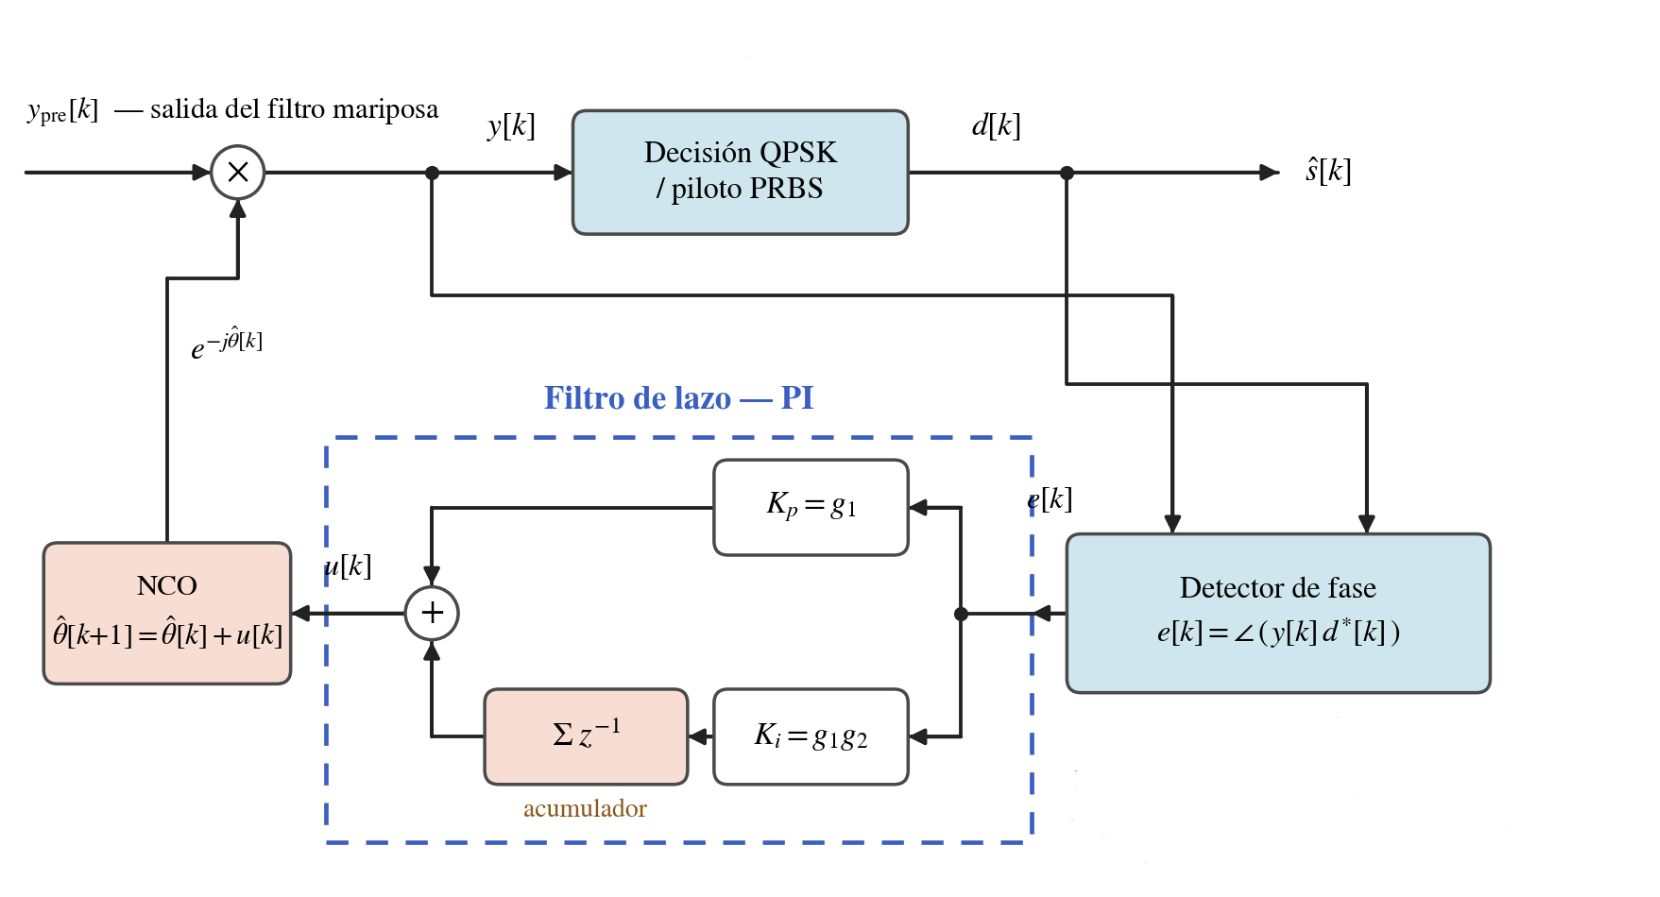
\includegraphics[width=0.95\linewidth]{ddlms_pll_recuperacionDeFase}
  \caption[Lazo de recuperaci\'on de fase]{%
    El lazo de fase dentro del bloque del ecualizador. La entrada
    $y_{\mathrm{pre}}[k]$ es la salida del filtro mariposa. El detector compara
    la se\~nal ya rotada contra la decisi\'on, que es el piloto PRBS durante el
    entrenamiento y la decisi\'on QPSK despu\'es. El filtro PI integra el error
    y el NCO acumula la fase estimada. El ecualizador se actualiza con el mismo
    error.}
  \label{fig:pll}
\end{figure}

Una alternativa a este lazo es un estimador feedforward tipo
Viterbi--Viterbi~\cite{mello2021}, que no necesita una etapa de enganche. En este trabajo se opt\'o por el lazo cerrado porque comparte el
error de decisi\'on con el ecualizador. De ese modo la rotaci\'on ya est\'a
corregida cuando el LMS actualiza los coeficientes, de manera que el
ecualizador no tiene que seguir al ruido de fase. Separar los dos bloques lo
obligar\'ia a compensar tambi\'en esa rotaci\'on, con una convergencia m\'as
lenta.

\paragraph{L\'imite te\'orico del lazo}
La \cref{eq:pll-filtro} es la misma rama proporcional e integral del lazo de
reloj, escrita de otra forma. Si se la desarrolla,
\[
  g_1\left[(1+g_2)\,\varepsilon[k] - \varepsilon[k-1]\right]
  = g_1\left(\varepsilon[k]-\varepsilon[k-1]\right) + g_1 g_2\,\varepsilon[k],
\]
queda claro que $K_p = g_1$ y $K_i = g_1 g_2$. Como es un lazo de tipo~2,
valen las mismas expresiones de la \cref{eq:lazo-2do}.

Como el error se calcula como $\arg(y\,d^{*})$, se tiene que $K_d = 1$. Con
$g_1 = 0{,}06$ y $g_2 = 0{,}025$, los parámetros característicos del lazo valen:
\begin{equation}
  f_n = \SI{197}{\mega\hertz},
  \qquad
  \zeta = \num{0.77},
  \qquad
  B_L = \SI{680}{\mega\hertz}.
  \label{eq:lazo-fase}
\end{equation}


\paragraph{Tolerancia al ancho de l\'inea}
El lazo no corrige la fase de forma instant\'anea. Su tiempo de respuesta
frente a un error de fase es del orden de
$\tau_L = 1/2B_L = \SI{0.74}{\nano\second}$. Lo que queda sin corregir en cada
instante es la fase que se acumul\'o durante los \'ultimos $\tau_L$ segundos.

La fase de un l\'aser es un proceso de Wiener, de modo que el incremento en un
intervalo $\tau$ es una variable aleatoria de media nula y varianza
proporcional a $\tau$. Para el ancho espectral combinado de los dos l\'aseres,
$\dnu_{\mathrm{tot}} = 2\dnu$,
\begin{equation}
  \sigma_\varphi^2
    = \operatorname{Var}\!\left[\varphi(t+\tau_L) - \varphi(t)\right]
    = 2\pi\, \dnu_{\mathrm{tot}}\, \tau_L
    = \frac{\pi\, \dnu_{\mathrm{tot}}}{B_L},
  \label{eq:var-fase}
\end{equation}
siendo entonces $\sigma_\varphi$ el valor eficaz del error de fase residual.

La \cref{eq:var-fase} contiene el compromiso de dise\~no del lazo. El error
residual crece con la ra\'iz del ancho de l\'inea y decrece con la ra\'iz del
ancho de banda del lazo. Ensanchar el lazo mejora el seguimiento de la fase,
pero tambi\'en deja entrar m\'as ruido aditivo al detector, efecto que esta
expresi\'on no contempla. El \'optimo surge al encontrar un equilibrio entre ambos mecanismos.

Mientras el error de fase instant\'aneo
se mantenga dentro del margen angular de QPSK, $\pm\ang{45}$
(\cref{cap:coherentes}), el lazo lo corrige. Cuando una excursi\'on lo supera,
el lazo se re-engancha desplazado un cuarto de vuelta y a partir de ah\'i
todos los s\'imbolos quedan decididos de manera err\'onea. Como el error de fase es gaussiano
de media nula, la frecuencia de esas excursiones es gobernada por la cantidad
de veces que cabe $\sigma_\varphi$ en los \ang{45}.

Esa ambig\"uedad de un m\'ultiplo de $\pi/2$ es tambi\'en la raz\'on por la
cual las m\'etricas se eval\'uan sobre las cuatro rotaciones posibles y sobre
el conjugado, tomando la de menor error.

El valor de $\sigma_\varphi$ al que se produce el quiebre no se deduce de
\eqref{eq:var-fase}, porque depende del presupuesto de error que el ruido
aditivo deja disponible. En el \cref{cap:tolerancias} se lo determina por
simulaci\'on, junto con el ancho de l\'inea m\'aximo tolerado y la ley de
escala con $B_L$.


\section{Sincronizaci\'on}
\label{sec:dsp-decision}

La cadena sincroniza la se\~nal recibida con la secuencia PRBS transmitida,
dos veces. La primera vez ocurre antes del ecualizador, para empezar la etapa
asistida por datos, y la segunda despu\'es, para poder comparar s\'imbolo a
s\'imbolo. Un receptor real no conoce la secuencia transmitida, as\'i que
estos dos bloques pertenecen al entorno de simulaci\'on y no a la cadena de recepci\'on. Por esa raz\'on
est\'an dibujados aparte en la \cref{fig:dsp-cadena}. Las m\'etricas se
calculan sobre los s\'imbolos posteriores a la ventana de convergencia del
ecualizador.

\section{Justificaci\'on del orden de los bloques}
\label{sec:dsp-orden}

\begin{itemize}

\item El ortogonalizador es el primer bloque porque compensa un error que se
vuelve irreversible si la recuperaci\'on de frecuencia act\'ua antes. Con
desbalance de cuadratura, la se\~nal compleja que se construye a partir de las
ramas, $z$, no es la deseada sino una combinaci\'on lineal en sentido amplio
de la se\~nal transmitida $s$ y de su conjugada,
\begin{equation}
  z = c_1\,s + c_2\,s^{*},
  \qquad
  c_1 = \tfrac{1}{2}\left(1 + \gamma e^{j\phi}\right),
  \qquad
  c_2 = \tfrac{1}{2}\left(1 - \gamma e^{j\phi}\right),
  \label{eq:iq-imbalance}
\end{equation}
donde $\gamma$ es el desbalance de ganancia entre I y Q y $\phi$ el
apartamiento de la cuadratura. El t\'ermino $c_2\,s^{*}$ es una imagen
conjugada. Si $s$ est\'a centrada en $+\Df$, la imagen est\'a en $-\Df$.

La imagen queda entonces exactamente en la frecuencia espejo de la se\~nal.
Eso es lo que permite cancelarla con una matriz real de $2\times2$ sin
memoria. El ortogonalizador aplica justamente eso, una operaci\'on
est\'atica sobre el par $(I, Q)$ con un solo par de coeficientes para toda la
se\~nal.

Ahora sup\'ongase que primero se corrige la frecuencia, es decir que se
multiplica todo por $e^{-j2\pi\Df t}$. Llamando $s' = s\,e^{-j2\pi\Df t}$ a la
se\~nal ya recentrada, y notando que
$s^{*}e^{-j2\pi\Df t} = s'^{*}\,e^{-j4\pi\Df t}$,
\begin{equation}
  z' = c_1\,s' + c_2\,s'^{*}\,e^{-j4\pi\Df t}.
  \label{eq:imagen-rotante}
\end{equation}
La imagen qued\'o en $-2\Df$ y dej\'o de estar en la frecuencia espejo. Una
matriz real de $2\times2$ sin memoria no puede cancelar un t\'ermino cuya fase
relativa rota. El ecualizador MIMO tampoco llega a seguirla. Sus coeficientes
se adaptan con una constante de tiempo de cien s\'imbolos, unos
\SI{3.1}{\nano\second}, mientras que la imagen completa una vuelta cada
\SI{0.25}{\nano\second} para el offset mayor de la \cref{tab:orden-gsop}.

El ortogonalizador tampoco puede estimar la correcci\'on en ese escenario.
Calcula un \'unico coeficiente de correlaci\'on $\E{r_I r_Q}$ promediado sobre
todo el bloque y aplica una \'unica correcci\'on est\'atica. Mientras la imagen
est\'a en el espejo, su aporte a esa correlaci\'on es un valor fijo y distinto
de cero. Cuando la imagen rota, el aporte promedia a cero y la estimaci\'on
falla.

La \cref{fig:orden-gsop} y la \cref{tab:orden-gsop} lo verifican en
simulaci\'on, inyectando un error de cuadratura conocido en los cuatro
carriles y comparando los dos \'ordenes con el resto de la cadena intacto.

\begin{figure}[H]
  \centering
  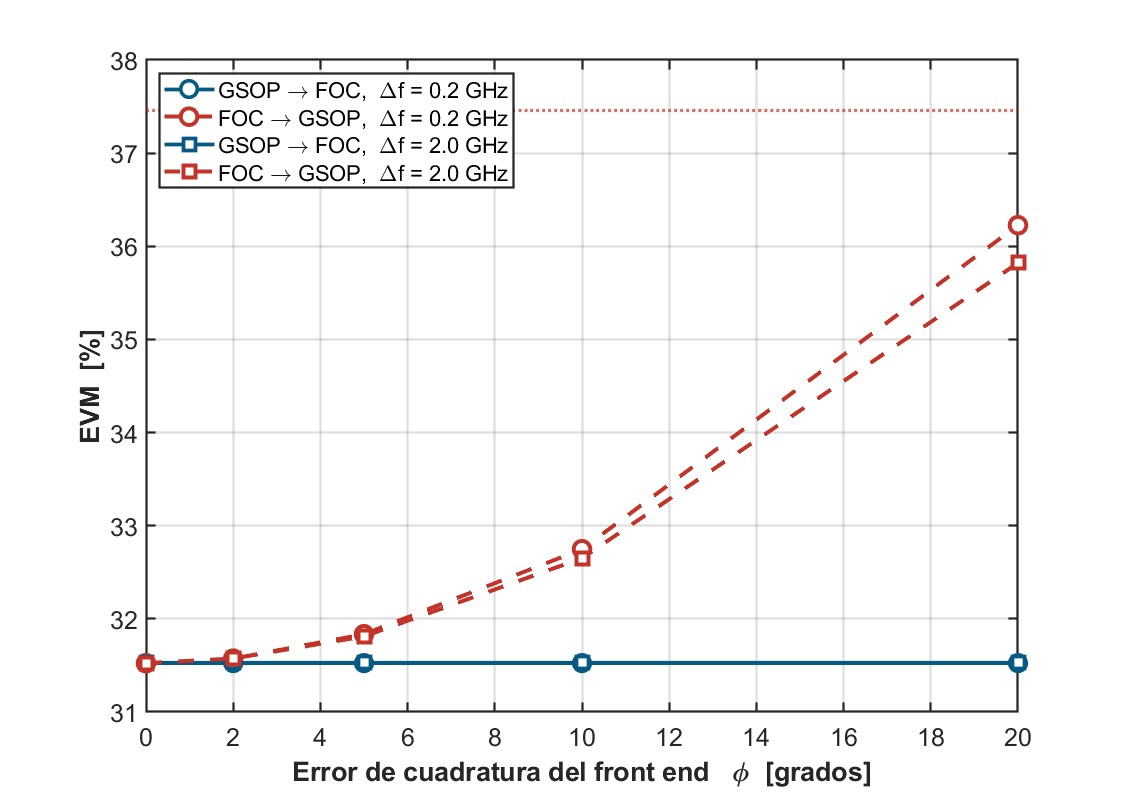
\includegraphics[width=0.92\linewidth]{orden_gsop_foc}
  \caption[Orden del ortogonalizador y el recuperador de frecuencia]{%
    EVM contra el error de cuadratura del front end, para los dos \'ordenes
    posibles y dos valores de offset de frecuencia. Con el orden correcto, en
    azul, las dos curvas quedan superpuestas y planas, de modo que el
    ortogonalizador remueve el desbalance por completo. Con el orden
    invertido, en rojo, el EVM crece con $\phi$. Las dos curvas quedan casi
    superpuestas entre s\'i aunque los offsets difieren un factor \num{10}, lo
    que muestra que la degradaci\'on no depende de $\Df$. La l\'inea punteada
    es el l\'imite HD-FEC.}
  \label{fig:orden-gsop}
\end{figure}

\begin{table}[H]
  \centering

  \begin{tabular}{cccccc}
    \toprule
    & \multicolumn{2}{c}{$\Df = \SI{0.2}{\giga\hertz}$}
    & \multicolumn{2}{c}{$\Df = \SI{2.0}{\giga\hertz}$} & \\
    \cmidrule(lr){2-3}\cmidrule(lr){4-5}
    $\phi$ & GSOP$\to$FOC & FOC$\to$GSOP & GSOP$\to$FOC & FOC$\to$GSOP
           & Penalidad \\
    \midrule
    \ang{0}  & \SI{31.52}{\percent} & \SI{31.52}{\percent} & \SI{31.53}{\percent} & \SI{31.53}{\percent} & \SI{0.00}{\dB} \\
    \ang{2}  & \SI{31.52}{\percent} & \SI{31.57}{\percent} & \SI{31.53}{\percent} & \SI{31.57}{\percent} & \SI{0.01}{\dB} \\
    \ang{5}  & \SI{31.52}{\percent} & \SI{31.83}{\percent} & \SI{31.53}{\percent} & \SI{31.81}{\percent} & \SI{0.09}{\dB} \\
    \ang{10} & \SI{31.52}{\percent} & \SI{32.75}{\percent} & \SI{31.53}{\percent} & \SI{32.65}{\percent} & \SI{0.33}{\dB} \\
    \ang{20} & \SI{31.52}{\percent} & \SI{36.23}{\percent} & \SI{31.53}{\percent} & \SI{35.82}{\percent} & \SI{1.21}{\dB} \\
    \bottomrule
  \end{tabular}
  \caption[Penalidad por invertir el orden de ortogonalizaci\'on y
           recuperaci\'on de frecuencia]{Penalidad por invertir el orden, a
           $\OSNR = \SI{14.4}{\dB}$ y \num{2e5} s\'imbolos.}
  \label{tab:orden-gsop}
\end{table}

Con el orden correcto el EVM es el mismo para todo $\phi$ entre \ang{0} y
\ang{20}, lo que indica que el ortogonalizador remueve el desbalance por
completo. Con el orden invertido el deterioro crece con $\phi$ hasta
\SI{1.21}{\dB}. La $\BER$ pasa de \num{7.6e-4} a \num{2.9e-3}, a un factor
\num{1.3} del umbral HD-FEC.

\item Por otro lado, hay una raz\'on para aplicar el filtro adaptado despu\'es
de la recuperaci\'on de frecuencia. El filtro RRC est\'a centrado en banda
base y tiene un ancho de banda de
$\Rs(1+\beta)/2 = \SI{19.2}{\giga\hertz}$. Con el Doppler del enlace la
se\~nal llega corrida hasta \SI{6}{\giga\hertz}, as\'i que un filtro aplicado
antes de corregir el offset recortar\'ia un borde del espectro de la se\~nal y
dejar\'ia pasar ruido por el otro. El estimador de cuarta potencia, en cambio,
no necesita que la se\~nal est\'e centrada. Trabaja sobre el espectro completo,
por lo que puede aplicarse primero. Recentrada la se\~nal, el filtro adaptado
act\'ua correctamente.

\item A su vez, el detector de error de muestreo mide la asimetr\'ia del pulso
en torno al instante de decisi\'on, de modo que trabaja mejor sobre el pulso
ya conformado por el filtro adaptado, con el ruido fuera de banda rechazado.
Pero adem\'as el detector calcula un producto entre muestras separadas medio
s\'imbolo y se queda con la parte real. Si la portadora todav\'ia gira a GHz,
esas muestras se comparan con fases distintas y el signo del error se vuelve
aleatorio. El detector necesita entonces las dos cosas, el pulso conformado y
la se\~nal ya recentrada en continua. Ubicarlo a continuaci\'on del filtro
adaptado, que a su vez va despu\'es de la recuperaci\'on de frecuencia,
satisface las dos condiciones.

\item Por \'ultimo, el ecualizador MIMO adaptativo es el \'unico bloque que
necesita una decisi\'on correcta para actualizarse. Todo lo que pueda
compensarse con un algoritmo que no dependa de la decisi\'on, es decir el
desbalance, el offset de frecuencia, el ruido fuera de banda y la fase de
muestreo, se remueve antes. As\'i el ecualizador arranca desde una
constelaci\'on ya reconocible y no tiene que converger a ciegas.

\end{itemize}

\section{Conclusiones}
\label{sec:dsp-conclusiones}

En este cap\'itulo se describieron los algoritmos de procesamiento digital
del receptor. Cada uno compensa una degradaci\'on distinta de las que el
enlace LEO--GEO y el front end introducen sobre la se\~nal.


El resultado central del cap\'itulo es el l\'imite de captura del estimador de
frecuencia. De los tres mecanismos analizados, el que predomina es el plegado
de Nyquist del tono de cuarta potencia, fijando un rango de $\Rs/4 = \SI{8}{\giga\hertz}$. Contra el requerimiento de \SI{6.0}{\giga\hertz} del \cref{cap:canal}
queda un \SI{33}{\percent} de margen.

Los dos lazos cerrados quedaron caracterizados por sus par\'ametros de segundo
orden. El de reloj,  por ser de tipo~2, sigue el desv\'io de frecuencia de muestreo 
debido al Doppler sin error
est\'atico. La aceleraci\'on del pase
le deja un error residual despreciable. El lazo de fase, a su vez, deja un
error de fase residual que escala como $\sqrt{\dnu_{\mathrm{tot}}/B_L}$.

El ecualizador MIMO cierra la cadena y absorbe los efectos que los dem\'as bloques
dejan. Al implementarse con filtros reales fraccionados en $T/2$, tiene la capacidad de compensar
el skew entre ramas y el desbalance de cuadratura residual, dos efectos que una
estructura estrictamente compleja no puede corregir. Su necesidad no depende del
canal. Entre los dos filtros RRC se interponen las respuestas del front end y
del conversor, de manera que el par transmisor--receptor no cumple el criterio
de Nyquist y deja interferencia entre s\'imbolos aun con el enlace ideal.

El orden en que se ejecutan no es arbitrario. La ortogonalizaci\'on se posiciona primero
porque el desbalance de cuadratura genera una imagen conjugada que, una vez
que la recuperaci\'on de frecuencia recentra la se\~nal, pasa a rotar y deja
de ser corregible con una operaci\'on est\'atica. El filtro adaptado se sit\'ua
despu\'es de la recuperaci\'on de frecuencia porque est\'a centrado en continua y
recortar\'ia una se\~nal desplazada en gigahertz. El detector de error de
muestreo le sigue filtro adaptado, que le entrega el pulso ya
conformado y sin el ruido fuera de banda. El ecualizador es el \'ultimo bloque porque es
el \'unico bloque que necesita una decisi\'on correcta para adaptarse. La
simulaci\'on confirma el primero de esos argumentos, con una penalidad de
\SI{1.21}{\dB} al invertir el orden frente a un error de cuadratura de
\ang{20}.

El \cref{cap:tolerancias} cuantifica por simulaci\'on los m\'argenes que este
cap\'itulo dej\'o planteados, entre ellos el ancho de l\'inea m\'aximo
tolerado y la velocidad de rotaci\'on del estado de polarizaci\'on que el
ecualizador alcanza a seguir.